\documentclass[10pt,a4paper]{article}
\usepackage[ngerman]{babel}
\usepackage[utf8]{inputenc}
\usepackage{amsmath}
\usepackage{amsfonts}
\usepackage{amssymb}
\usepackage{marvosym}
\usepackage{graphicx} % Allows for eps images
\usepackage{hyperref} %Links
\usepackage[noabbrev]{cleveref}
\usepackage{url}
\usepackage{bookmark}
\renewcommand{\UrlFont}{\small\tt} %smaller font for urls
\usepackage[a4paper,lmargin={2.5cm},rmargin={2.5cm},tmargin={2.5cm},bmargin = {2.5cm}]{geometry}
\usepackage{siunitx} % Zur einfachen Verwendung von SI-Einheiten und korrekte Rundungen
\sisetup{
        locale = DE , % Deutsche Dezimalzeichen u.a.
        per-mode = symbol, 
    }


%Some other shit
\usepackage{float}
%\floatstyle{boxed}
\restylefloat{figure}
\usepackage{wrapfig}

\usepackage{listings}
\usepackage{xcolor}

\definecolor{codegreen}{rgb}{0,0.6,0}
\definecolor{codegray}{rgb}{0.5,0.5,0.5}
\definecolor{codepurple}{rgb}{0.58,0,0.82}
\definecolor{backcolour}{rgb}{235, 235, 235}

\lstdefinestyle{mystyle}{
    backgroundcolor=\color{backcolour},   
    commentstyle=\color{codegreen},
    keywordstyle=\color{magenta},
    numberstyle=\tiny\color{codegray},
    stringstyle=\color{codepurple},
    basicstyle=\ttfamily\footnotesize,
    breakatwhitespace=false,         
    breaklines=true,                 
    captionpos=b,                    
    keepspaces=true,                 
    numbers=left,                    
    numbersep=5pt,                  
    showspaces=false,                
    showstringspaces=false,
    showtabs=false,                  
    tabsize=2
}
\lstset{style=mystyle}
\lstset{literate=%
  {Ö}{{\"O}}1
  {Ä}{{\"A}}1
  {Ü}{{\"U}}1
  {ß}{{\ss}}1
  {ü}{{\"u}}1
  {ä}{{\"a}}1
  {ö}{{\"o}}1
}
\usepackage[title,titletoc]{appendix}
\renewcommand{\appendixtocname}{Anhang}
\renewcommand{\appendixpagename}{Anhang}

\linespread{1.1}

\begin{document}

\pagenumbering{Roman}

%Metadaten
\title{Fortgeschrittenenpraktikum\\ Kurzversuch 6:\\ Fourier-Transform-Spektroskopie }
\author{Nico Kalogerakis \\ Léonie Lanz}

\maketitle

\begin{figure}[H]
       \centering
       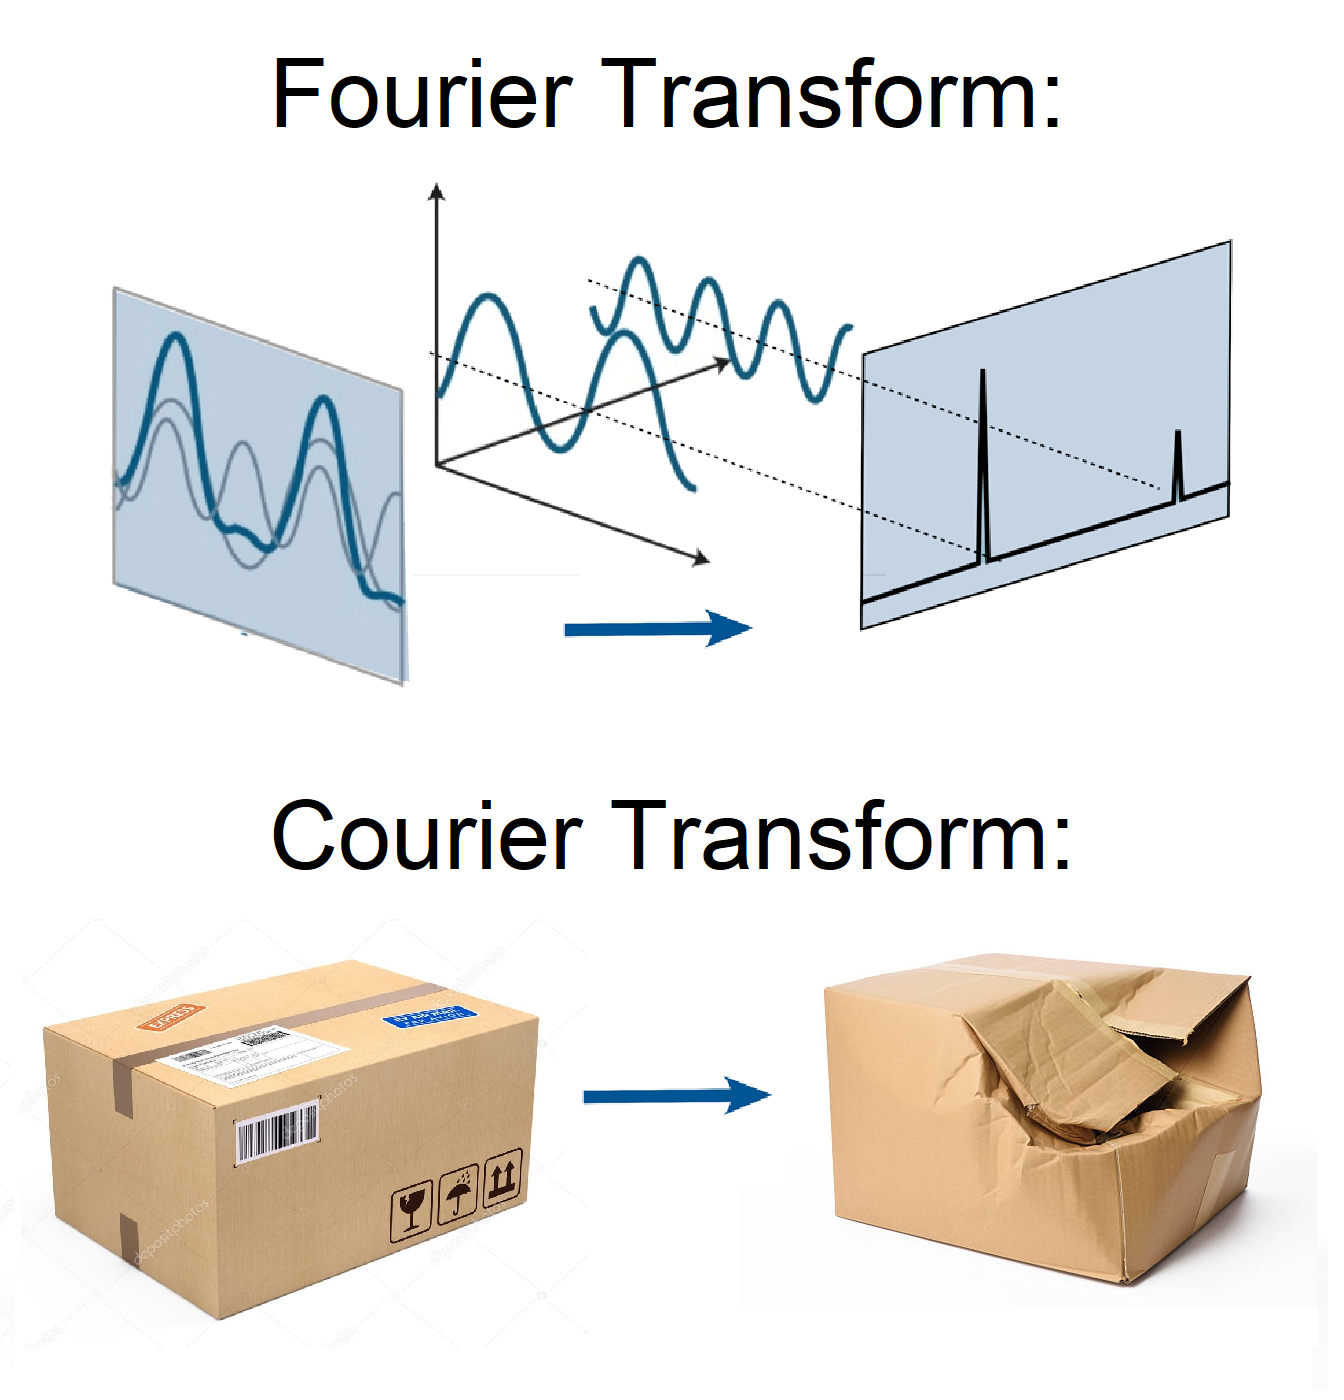
\includegraphics[scale=0.12]{img/FFT meme.png}
\end{figure}
\newpage

\tableofcontents
\vfill
\newpage

\pagenumbering{arabic}

\section{Einleitung}
%Aufgabenstellung, Ziel der Messungen
Der Kurzversuch 6 - Fourier-Transform-Spektroskopie dient der Einführung in das universelle Konzept der Fourier-Transform-Spektroskopie und dem Erlernen des Programmierens einer Auswertungsroutine.\\
Bei Fourier-Transform-Spektroskopie werden Spektren durch Messungen der Kohärenz der Strahlungsquelle bestimmt. Dafür wird die Intensität in Abhängigkeit der Zeit gemessen und das Spektrum durch die namensgebende Fouriertransformation berechnet.\\
Zu didaktischen Zwecken wird hier sichtbares Licht verwendet, anstelle von dem gängigen Infrarotlicht.
Ziel des Experiments ist sowohl das Spektrum einer Weißlichtlampe, als auch die Absorptionsspektren von einem Interferenz-Filter und von molekularem Iod zu bestimmen.\\
Dafür wird zuerst die zeitliche Kohärenzfunktion für die Weißlichtquelle ermittelt, aus der dann durch eine Fourier-Transformation auf das Spektrum der Quelle geschlossen wird. 

\section{Theoretische Grundlagen}
%Kurze Zusammenfassung der wichtigsten überlegungen (Formeln), die zum Verständnis des Versuches notwendig sind
%Für Details: Hinweise auf die Literatur
\subsection{Weißlichtspektrum}

Die im Versuch verwendete Weißlichtquelle ist eine Weißlicht-LED. Ihr Spektrum setzt sich typischerweise aus zwei charakteristischen Komponenten zusammen: Eine blaue Leuchtdiode emittiert Licht im Bereich von ca. \qty{440}{nm} bis \qty{480}{nm}, welches teilweise von einem Farbstoff (Phosphor) absorbiert und als breitbandiges, gelbliches Licht im Bereich von ca. \qty{550}{nm} bis \qty{600}{nm} reemittiert wird. Da Blau und Gelb Komplementärfarben sind, ergibt die überlagerung dieser Anteile für das menschliche Auge den Eindruck von weißem Licht. Apparative Einflüsse können zudem zu „spektralen Löchern“ führen, wie sie im Versuchsaufbau oft bei \qty{604}{nm} und \qty{617}{nm} beobachtet werden \cite{5}.

\subsection{Interferometrie}
Interferometrie ist das Prinzip, mithilfe von Interferenzphänomenen Messungen zu vollziehen. Im Allgemeinen bezieht sich Interferometrie auf Wellen jeglicher Art, hier beschäftigen wir uns aber nur mit den elektromagnetischen - dem Licht \cite{1}.\\\\
Das Michelson-Interferometer, das auch in diesem Versuch einen zentrale Rolle spielt, ist ein Zwei-Strahl-Interferometer in dem durch einen Strahlteiler zwei identische Strahlen erzeugt werden. Nur wenn die Kohärenzbedingung für die beiden Strahlen zutrifft, also nur wenn zwei sich zeitlich gleichverhaltende ebene Wellenfronten aufeinander treffen, erscheint das Interferenzmuster streifenförmig \cite{2}.\\
Die optische Weglängendifferenz $\Delta s_{opt}$ hängt beim Michelson-Interferometer sowohl von der geometrischen Weglänge der Arme $s_1, s_2$ als auch von den Brechzahlen $n_1, n_2$ der durchlaufenen Medien ab: $\Delta s_{opt} = n_1s_1 - n_2s_2$. Für den Betrieb als Fourier-Transform-Spektrometer wird das System so justiert, dass die Detektoreinheit nur einen Bereich des Interferenzmusters vermisst, in dem eine einheitliche Phasendifferenz vorherrscht („ein Streifen“). Eine Variation der Weglängendifferenz um $\Delta x$ resultiert dabei in einer Änderung des optischen Weges um $2\Delta x$, da das Licht den veränderten Weg doppelt (hin und zurück) durchläuft \cite{1}.\\

\subsection{Kohärenz und Autokorrelation}
Es wird zwischen räumlicher und zeitlicher Kohärenz unterschieden, wenn es um die Interferenzfähigkeit von Wellen geht. Zeitliche Kohärenz ist die Fähigkeit von Wellen mit unterschiedlichen zurückgelegten optischen Wegen zu interferieren, also ist die Phasenbeziehung bezüglich der Zeitachse fest trotz möglicher Variation der Phasenbeziehung bezüglich der Raumachse. Für die zeitlich stationären Interferenzmuster, die wir bei einem Michelson-Interferometer betrachten, muss zeitliche Kohärenz der überlagernden Wellen vorliegen\\
Es gibt eine maximale Zeitraum $\Delta t$, in dem zeitliche Kohärenz vorliegt -- die Kohärenzzeit.\\\\
Das genaue Maß der Kohärenz zweier Wellen lässt sich durch die Kohärenzfunktion beschreiben.
Wir betrachten das einfallende Wellenfeld an einem festen Punkt und aufgeteilt in zwei Anteile mit gleich großer Amplitude:
$$E(t)=E_1(t)+E_2(t).$$
Die resultierende Intensität der überlagerung sieht in unserem Fall von zwei gleichen Wellen folgendermaßen aus \cite{2}:
\begin{equation}
I(\Delta t)=\langle(E_1+E_2)(E_1+E_2)^*\rangle=I_1+I_2+2Re\langle E^*_1E_2 \rangle =I_1+I_1+2Re\Gamma(\Delta t).
\end{equation}
Der dritte Term $\Gamma(\Delta t)$ beinhaltet die Intensität des korrelierten Teils der überlagerung und nennt sich (Selbst-) Kohärenzfunktion oder auch Autokorrelationsfunktion, weil sie der Autokorrelation des Lichtfeldes $E_1(t)$ entspricht \cite{2}:
\begin{equation}
\Gamma(\Delta t)=\langle E^*_1(t)\cdot E_1(t+\Delta t)\rangle = \lim_{T\to\infty}\frac{1}{T}\int^{T/2}_{-T/2}E^*_1(t)\cdot E_1(t+\Delta t)dt.
\end{equation}

Ein Maß für die Interferenzfähigkeit ist die Kohärenzlänge $l_K$, welche die räumliche Ausdehnung der Kohärenz beschreibt und über die spektrale Bandbreite $\Delta\lambda$ mit der Wellenlänge $\lambda$ verknüpft ist: $l_K = \lambda^2 / \Delta\lambda$. 
In der experimentellen Praxis ist die Kohärenzfunktion $\Gamma(\Delta t)$ nicht direkt zugänglich. Stattdessen wird der Kontrast $K$ (oder Sichtbarkeit) des Interferenzmusters herangezogen, definiert über die Intensitätsmaxima und -minima $I_{max}, I_{min}$ \cite{2}:
\begin{equation}
K(\Delta t) = \frac{I_{max} - I_{min}}{I_{max} + I_{min}}.
\end{equation}
Für den Spezialfall gleich intensiver Teilwellen entspricht die Kontrastfunktion exakt dem Betrag des komplexen Kohärenzgrades $|\gamma(\Delta t)|$ \cite{2}.


\subsection{Fourier-Spektroskopie}
Das Funktionsprinzip der Fourier-Transform-Spektroskopie (FTS) beruht auf der Erkenntnis, dass die experimentell bestimmbare Autokorrelationsfunktion $I(\Delta t)$ die Fourier-Transformierte der spektralen Energiedichte $W(\omega)$ darstellt. 

Geht man von einem Wellenfeld mit beliebig vielen Frequenzkomponenten aus, lässt sich das elektrische Feld als Integral beschreiben:
\begin{equation}
E(t) = \frac{1}{2\pi} \int_{0}^{\infty} E_0(\omega)e^{-i\omega t}d\omega.
\end{equation}
Unter der Annahme einer symmetrischen spektralen Energiedichte ($W(\omega) = W(-\omega)$) ergibt sich für den interferierenden Teil der Intensität $\Delta I(\Delta t)$ nach dem Wiener-Khinchin-Theorem der Zusammenhang:
\begin{equation}
\Delta I(\Delta t) = \frac{1}{2\pi} \int_{-\infty}^{\infty} W(\omega) e^{-i\omega \Delta t} d\omega.
\end{equation}
Durch eine numerische Rücktransformation (Inverse Fourier-Transformation) kann somit aus dem gemessenen Interferogramm das gesuchte Spektrum extrahiert werden:
\begin{equation}
W(\omega) = \int_{-\infty}^{\infty} \Delta I(\Delta t) e^{i\omega \Delta t} d(\Delta t).
\end{equation}\\
In der Realität ist die spektrale Auflösung $\Delta\nu$ jedoch durch die maximale zeitliche Verzögerung $\Delta t_{max}$ begrenzt, die experimentell durch den Verfahrweg des Spiegels erreicht werden kann: $\Delta\nu = 1/\Delta t_{max}$. Zudem begrenzt das Nyquist-Shannon-Abtasttheorem die maximal messbare Frequenz $\nu_{max}$ durch das Zeitintervall $t_{sampl}$ zwischen zwei Messpunkten: $\nu_{max} = 1/(2 t_{sampl})$ \cite{2}.


\section{Experimenteller Aufbau}
\begin{figure}[!h]
	\centering
	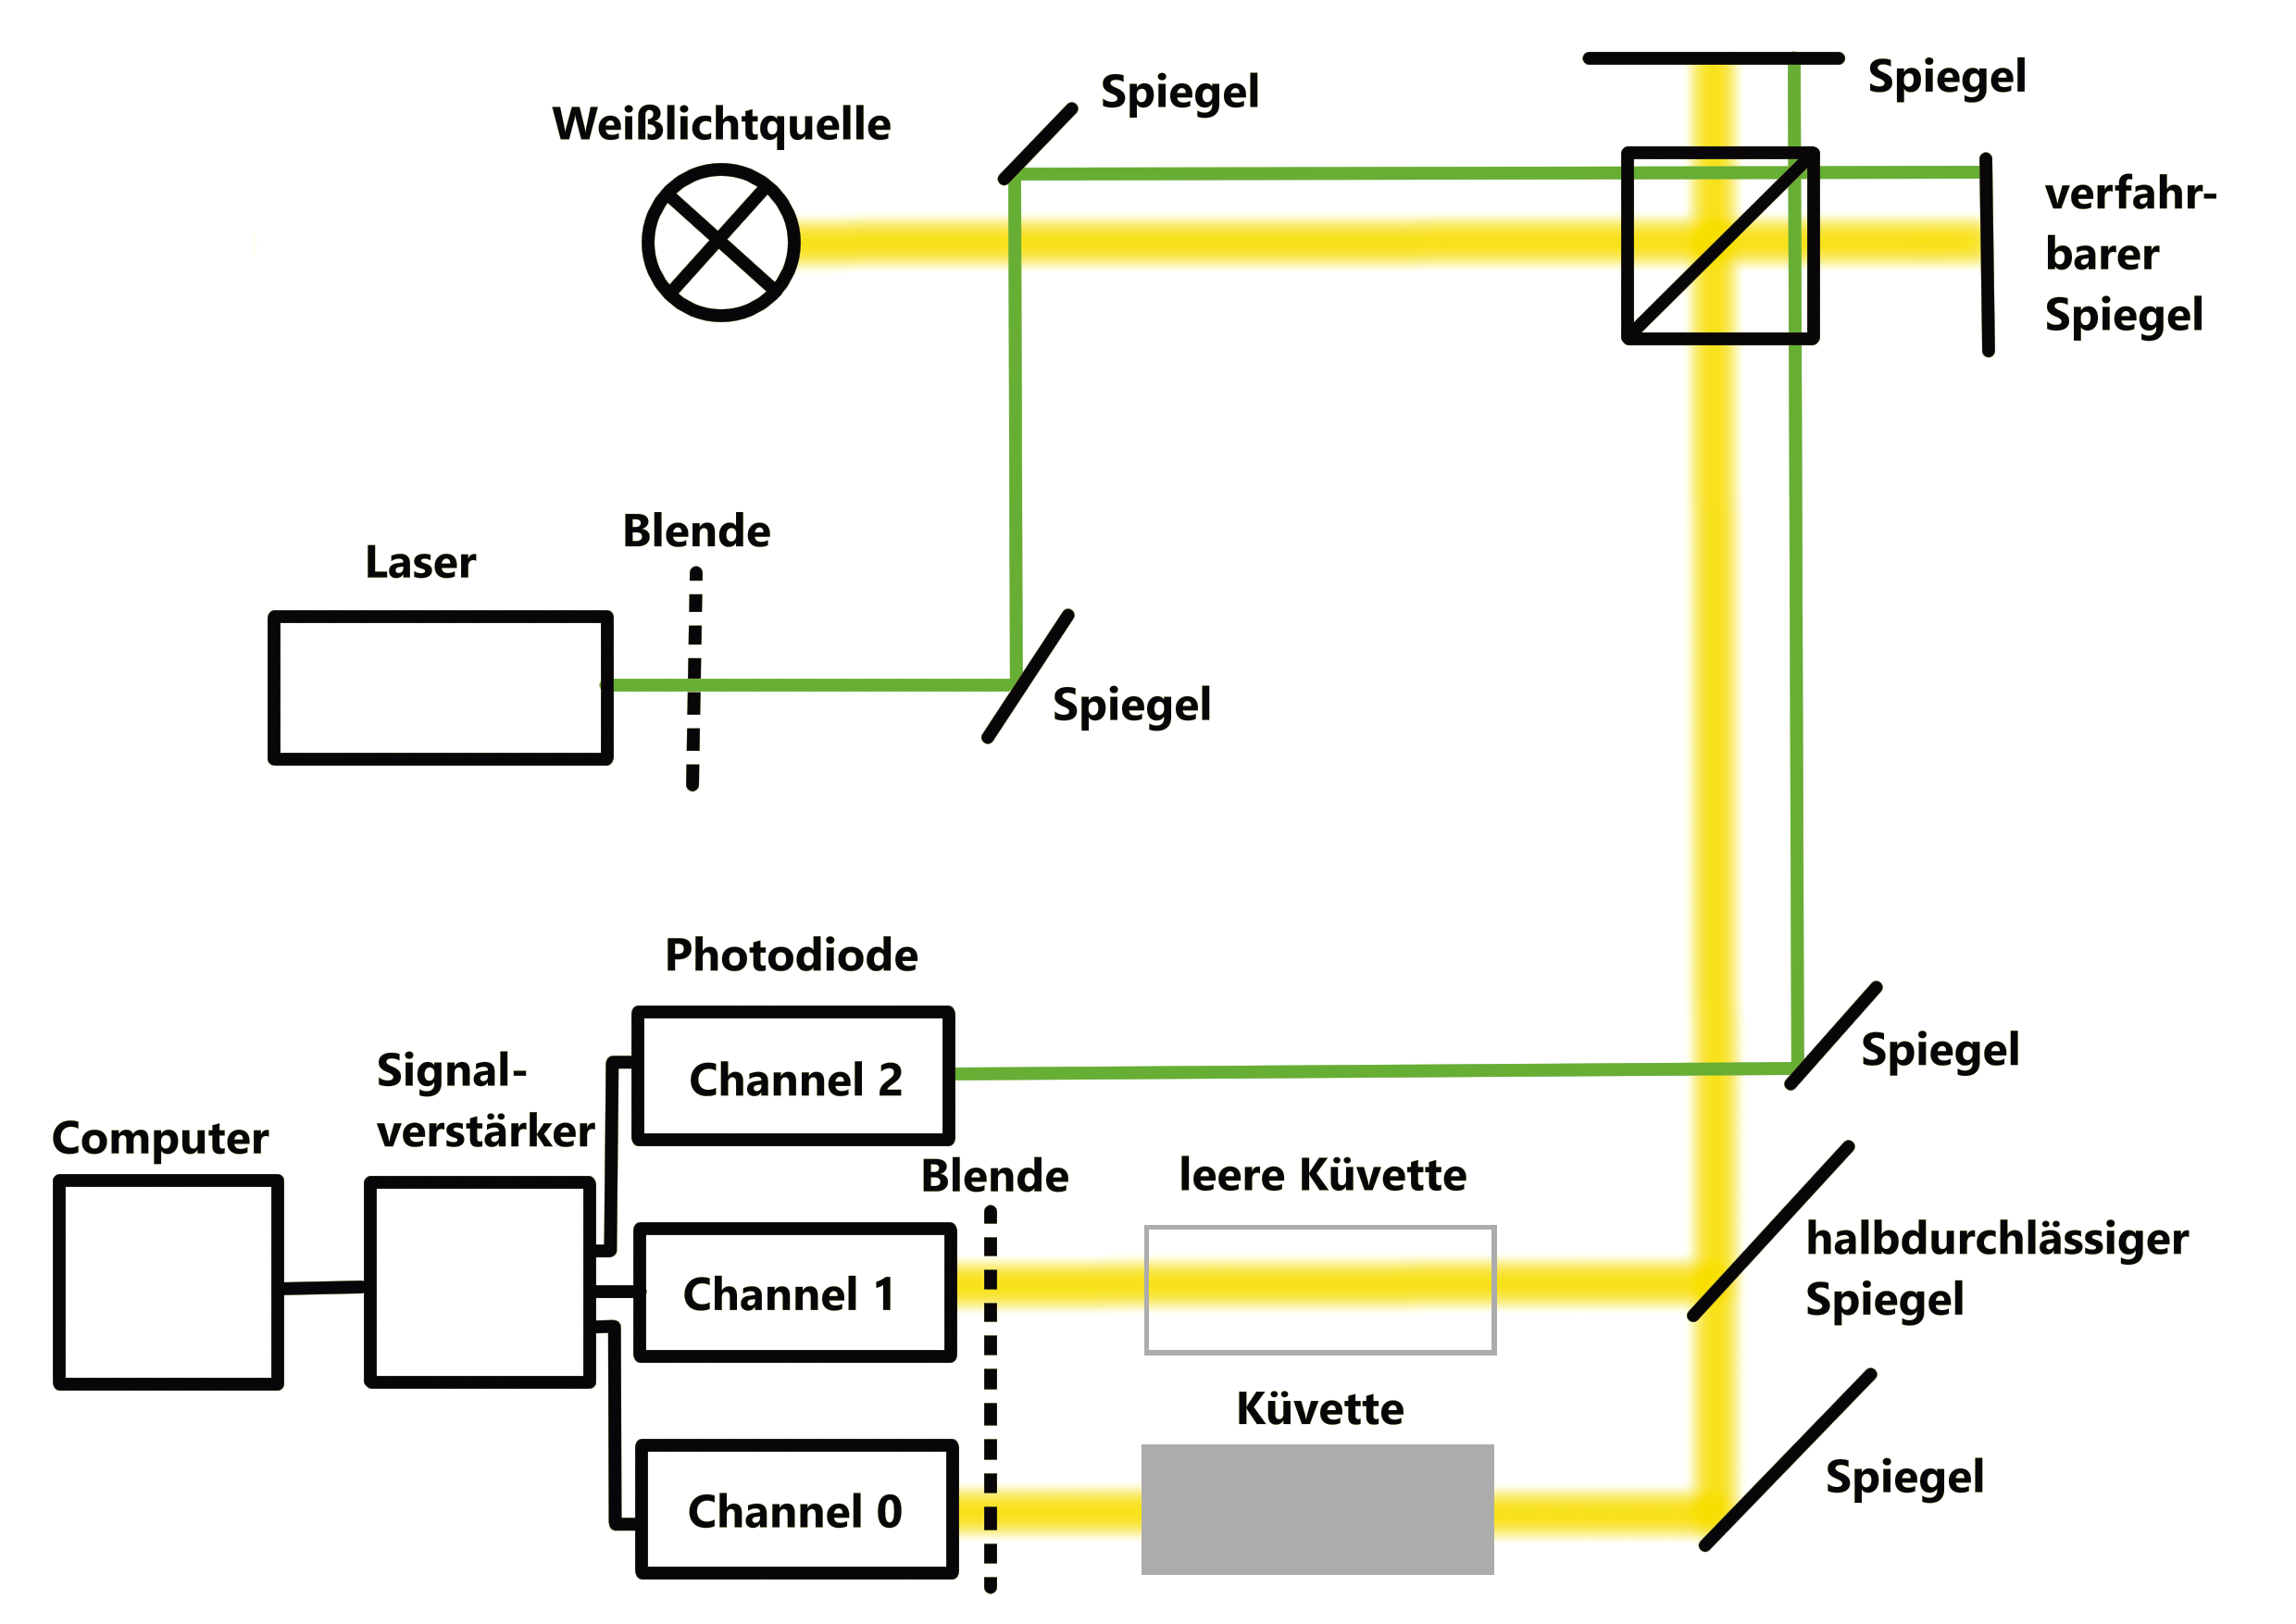
\includegraphics[width=0.75\linewidth]{img/versuchsaufbau.png}
	\caption{Schematischer Aufbau des Fourier-Transform-Spektrometers.}
	\label{fig: michint}
\end{figure}

Das Fourier-Transform-Spektrometer, das in diesem Versuch verwendet wird, besteht hauptsächlich aus einem Michelson-Interferometer. Wie in \autoref{fig: michint} zu sehen, werden in das Michelson-Interferometer zwei Strahlengänge gleichzeitig eingekoppelt: zum einen der zu untersuchende Weißlichtstrahlengang, zum anderen der Laserstrahlengang, der der Kalibrierung der optischen Weglängendifferenz des Interferometers dient.\\
Die Weißlichtquelle hier ist eine Weißlicht-LED und der Laser ist ein frequenzverdoppelter diode-pumped solid-state-Laser mit einer Wellenlänge von $\lambda_L=\qty{532}{nm}$.\\\\
Das Michelson-Interferometer teilt die einfallenden Lichtbündel in zwei identische Lichtstrahlen auf, die beide über Spiegel wieder zurückgeworfen werden. Einer der beiden Spiegel des Interferometers lässt sich über einen Linearverschiebetisch angetrieben von einem Schrittmotor bewegen.\\
Nach dem  Durchlaufen des Interferometers wird der Strahlengang des Lasers auf eine einzelne Fotodiode gelenkt, während der Weißlichtstrahl erneut durch einen halbdurchlässigen Spiegel geteilt wird. Einer der beiden Weißlichtstrahlen wird direkt auf eine Fotodiode gelenkt, der andere durchläuft die zu untersuchenden Proben, bevor er auch auf eine Fotodiode trifft.\\
Die, von den drei Photodioden kommenden, Signale werden durch Operationsverstärker verstärkt und invertiert um an den Dynamikbereich eines Analog-Digital-Wandlers angepasst zu werden. Dann werden die Signale erst an den AD-Wandler und von dort an einen Computer weitergeleitet.\\\\
Die Steuerung des Motors und die Aufnahme der Daten erfolgt über ein Python GUI.\\
Die kleinstmögliche Schrittgröße des Schrittmotors beträgt rechnerisch \qty{50,5}{nm}. Allerdings ist die Bewegung des Verschiebetisches nicht exakt linear, was in der Auswertung berücksichtigt werden muss. Außerdem braucht der Antrieb ein gewisses Umkehrspiel, was kompensiert werden kann, indem Änderungen der Bewegungsrichtung nur in einer guten Entfernung von dem Startpunkt der Messungen aus vorgenommen werden - hier reichen etwa 1000 Schritte.\\\\
Bevor die Messungen gestartet werden, muss die Position Null des Motors auf die Mitte des Interferenzmusters gesetzt werden.

\section{Versuchsdurchführung}
Fourier-Transform-Spektroskopie basiert darauf, die Weglängendifferenz der beiden Teilarme des Interferometers kontrolliert zu variieren. Durch die Variation der Weglängendifferenz wird auch die zeitliche Verzögerung der beiden Teilstrahlen $\Delta t$ variiert.\\\\
Der Versuch lässt sich in zwei Abschnitte aufteilen. Im ersten Messdurchlauf ist ein Interferenz-Filter die Probe, im Zweiten eine Küvette mit molekularem Iod. Das Ziel ist es die Veränderung des Weißlichtspektrums unter Einfluss der beiden Proben zu untersuchen.\\\\
Nach der Justage wird der Interferenzfilter in einen der beiden Weißlichtstrahlengänge eingebaut. Der Schlitten des Spiegels wird vom Nullpunkt bis zu Motorposition -6000 gefahren und dann 1000 Schritte zurückgefahren um das mögliche Spiel des Motors beim Umkehren des Schlittens zu verhindern.\\
Nun erfolgt eine Messung mit 10000 Schritten -- von Motorposition -5000 bis 5000 -- mit folgenden Parametern in der Software: 20 Werte pro Messpunkt, 1 Schritt pro Messpunkt und einer Abklingzeit von \qty{10}{ms}.\\
Für den zweiten Messdurchlauf wird der Interferenzfilter durch die Glasküvette mit dem Iod ersetzt. An die Küvette wird eine Heizspannung von \qty{22,5}{V} angesetzt, sodass die Küvettentemperatur $76,7\pm 0,1$°C beträgt. In den Referenz-Weißlichtstrahlengang wird eine leere Glasküvette eingebaut.\\
Jetzt wird der Schlitten wieder zuerst auf Position -6000, dann auf -5000 gebracht. Nun folgt wieder eine Messung nach den oben genannten Parametern.

\section{Auswertung der Messungen}

\subsection{Datenstruktur und Vorverarbeitung}

\subsubsection{Datenformat}
Die vom Computer verwendete Software erzeugt pro Messung für jeden Messkanal eine Datei, die entsprechend des Signalursprungs benannt ist. Hier werden, für jeden der drei aufgenommenen Datensätze, drei Dateien erzeugt \footnote{Channel 0: Probe, Channel 1: Referenz, Channel 2: Laser}. 
Dort werden die Messwerte des jeweiligen Kanals für jeden vom Linearantrieb angefahrenen Messpunkt als ASCII-Dateien gespeichert. Diese sind in 10000 Zeilen angeordnet, da von -5000 bis 4999 insgesamt 10000 Positionen ab- gefahren werden. Pro Position wurden 20 Messwerte aufgenommen. Die erste Spalte enthält immer die Motorposition in Schritten, die darauffolgenden dann die eigentlichen Messwerte.\\
Zu Beginn der Datenanalyse werden die Dateien des Lasersignals und später auch die des Weißlichtsignals in das Auswertungsprogramm importiert.

\subsubsection{Mittelung}
Der erste Schritt im Skript ist die Mittelwertbildung der 20 Messwerte pro Position, um das Signal-zu-Rausch-Verhältnis zu verbessern.

\subsubsection{Vorverarbeitung Code}

\begin{lstlisting}[language=Python, caption=Vorverarbeitung]
def load_data(filepath):
       data = np.loadtxt(filepath)
       positions = data[:, 0]
       measurements = data[:, 1:20]  # N Spalten mit Messwerten
       return positions, measurements
   
def average_measurements(measurements):
       return np.mean(measurements, axis=1)
\end{lstlisting}


\subsection{Kalibrierfunktion}
Da die mechanische Bewegung des Linearverschiebetisches nicht exakt linear verläuft und der Antrieb zudem ein gewisses Umkehrspiel aufweist, ist eine numerische Korrektur der Ortsachse nötig. Die Kalibrierung erfolgt anhand des Laser-Interferogramms (Kanal 2), da dessen Wellenlänge ($\lambda_{L}=\qty{532}{nm}$) exakt bekannt und die Form des Interferogramms genau vorhersagbar ist.\\
Die Bestimmung der Kalibrierfunktion gliedert sich in folgende Schritte:

\begin{itemize}
       \item Interpolation zur Erhöhung der Abtastrate: Um die Genauigkeit der Peak-Suche zu steigern, werden die gemittelten Laserdaten zunächst um den Faktor 10 interpoliert. Hierbei kommt eine 'Univariate-Spline'-Funktion vierten Grades aus der SciPy-Bibliothek zum Einsatz. Die Wahl eines Splines vierten Grades begründet sich dadurch, dass sich die Extrema über die Nullstellen der Ableitung mathematisch besonders präzise bestimmen lassen. Graphisch wird das in \autoref{fig:LaserDatenInterpolationvsOriginaldaten} gezeigt.
       \item Identifikation der Ist-Positionen $P_{ist}$: Mithilfe der Funktion `argrelextrema` werden die Maxima des interpolierten Lasersignals identifiziert. Diese Maxima markieren die realen Positionen $P_{ist}$ des Spiegels im Interferogramm. In \autoref{fig:LaserDatenInterpolationmitMaxima} sieht man die interpolierten Laserdaten überlagert mit den Maxima.
       \item Berechnung der Soll-Positionen $P_{soll}$ via linearer Regression: Im idealen Fall einer völlig linearen Bewegung müssten diese Maxima in äquidistanten Abständen liegen. über eine lineare Regression der Form $P_{soll}(i)=a\cdot i+b$ werden daher die theoretischen Soll-Positionen für jedes Maximum bestimmt. Diesen Fit sieht man in \autoref{fig:Kalibrierfunktion}.
       \item Erzeugung der kontinuierlichen Korrekturfunktion: Die lokale Abweichung der Motorbewegung berechnet sich an den Stützstellen zu $\Delta(i)=P_{soll}(i)-P_{ist}(i)$. Um diese Korrektur auf den gesamten Datensatz und beliebige Motorpositionen anwenden zu können, wird der diskrete Verlauf von $\Delta$ erneut interpoliert. Das resultierende Funktions-Objekt stellt somit für jeden Messpunkt einen individuellen Korrekturwert zur Linearisierung der Ortsachse bereit. Diesen Korrekturwert kann man daraufhin auf die ursprünglichen Laserdaten anwenden, was man in \autoref{fig:KorrekturderMotorposition} sieht.
\end{itemize}

\subsubsection{Kalibrierfunktion Code}

\begin{lstlisting}[language=Python, caption=Hilfsfunktionen für die Kalibrierfunktion]
def interpolate(x, y, factor=10): #for x positions und y avergae_measurements
       f_interpol = make_interp_spline(x, y, k=3)
       x_new = np.linspace(x.min(), x.max(), len(x)*factor)
       y_new = f_interpol(x_new)
       return x_new, y_new
   
def find_extrema(y):
       peaks = argrelextrema(y, np.greater)[0]
       troughs = argrelextrema(y, np.less)[0]
       extrema_list = []
       for i, j in zip(peaks, troughs):
           extrema_list.append(i)
           extrema_list.append(j)
   
       extrema_array=np.array(extrema_list)
   
       return extrema_array, peaks
   
def linear_fit(extrema):
       r = np.linspace(0, len(extrema)-1, len(extrema))
       fit = linregress(r, extrema)
       return r, fit
\end{lstlisting}

\begin{lstlisting}[language=Python, caption=Kalibrierfunktion]
def korrekturfunktion(data):
       # Analyse der Laser-Daten:
       file_path = "data/"+data+"/Data Channel 2.dat"
       positions, measurements = load_data(file_path)
       mean_data_laser = average_measurements(measurements)
       
       # Erste Interpolation der Laser-Daten
       x_new, y_new = interpolate(positions, mean_data_laser, factor=10)
   
       # Bestimmung der Extrema
       _, extrema_array = find_extrema(y_new)
       maxima_positions = x_new[extrema_array]
       print("maxima menge = ",len(maxima_positions))
       
       # Kalibrierfunktion bestimmen
       _, fit = linear_fit(maxima_positions)
   
       P_soll = np.empty(len(maxima_positions), dtype=int)
       P_ist = maxima_positions
       for i in range(len(maxima_positions)):
           P_soll[i] = fit.intercept + fit.slope*i
       delta = P_soll - P_ist
       delta_interpolate = make_interp_spline(P_ist, delta, k=3)
   
       return delta_interpolate, fit.slope
\end{lstlisting}

\subsubsection{Graphen}

\begin{figure}[H]
       \centering
       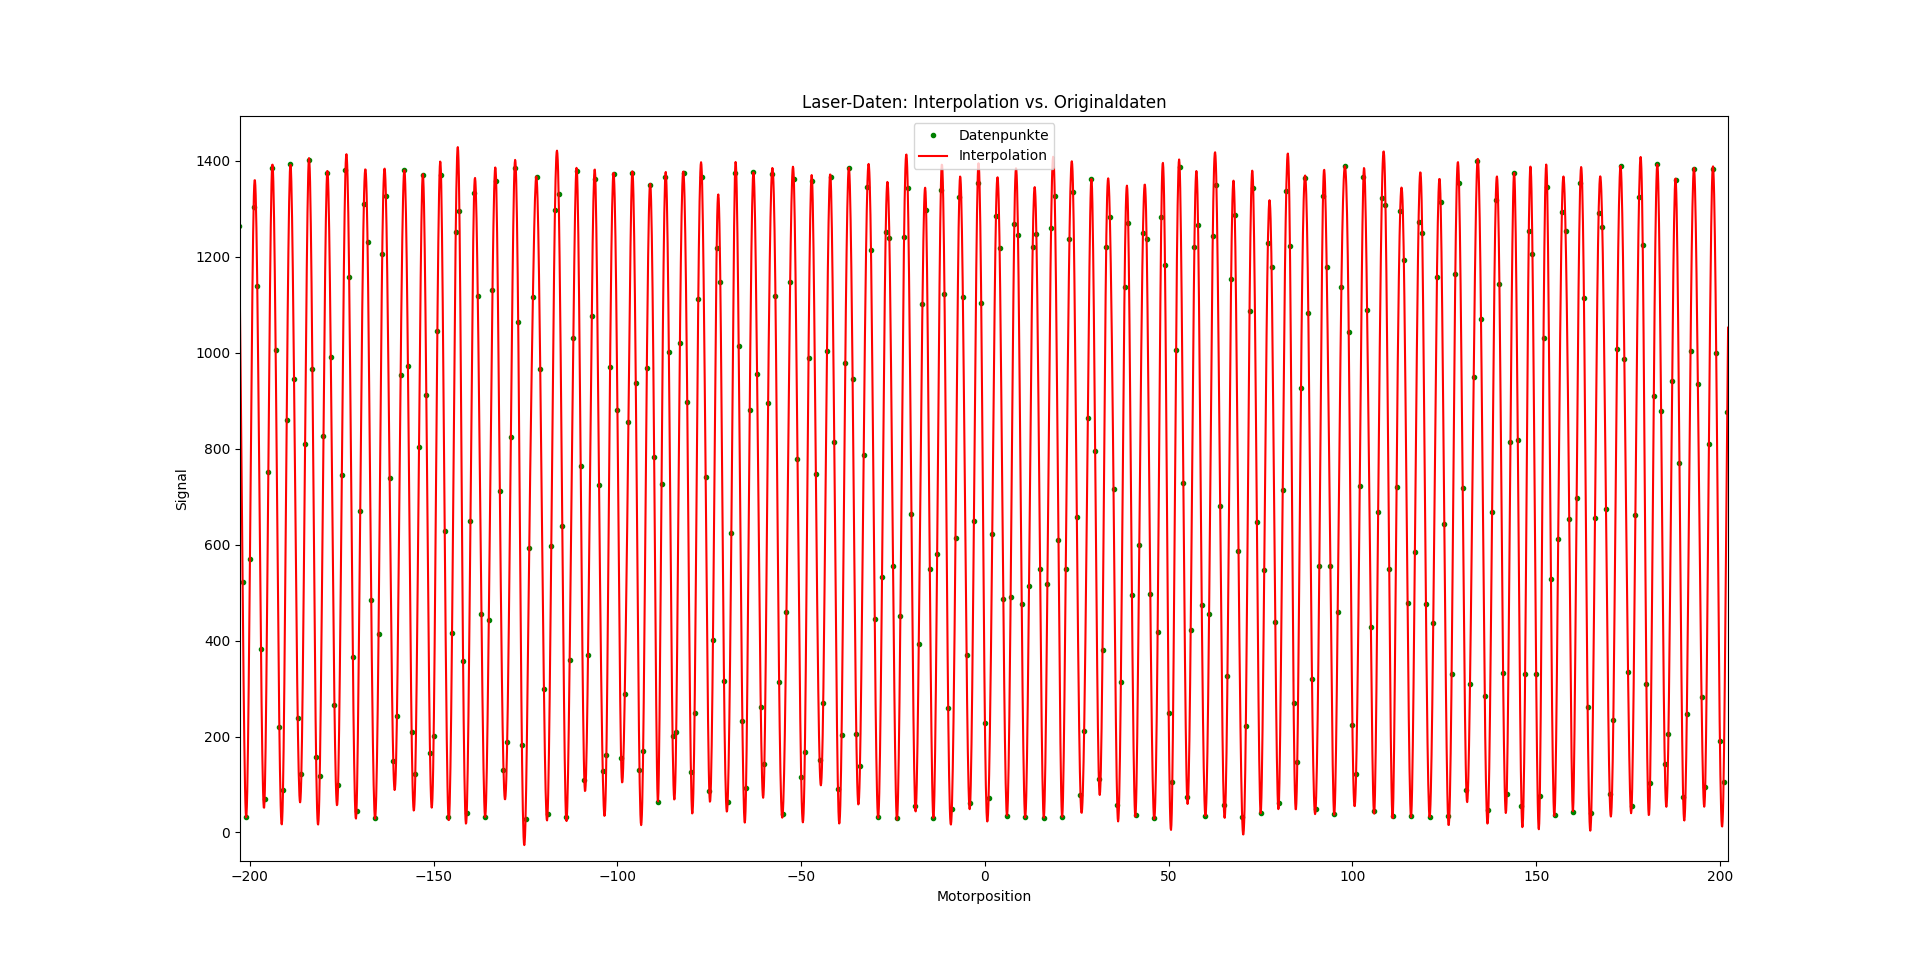
\includegraphics[width=1\linewidth]{img/Laser Daten Interpolation vs Originaldaten.png}
       \caption{Die Interpolierten Laser Daten (in rot) überlagert mit den Originaldaten (grüne Punkte.)}
       \label{fig:LaserDatenInterpolationvsOriginaldaten}
       %grafiken würde ich erst mit einer korrigierten Korrekturfunktion besser machen
\end{figure}

\begin{figure}[H]
       \centering
       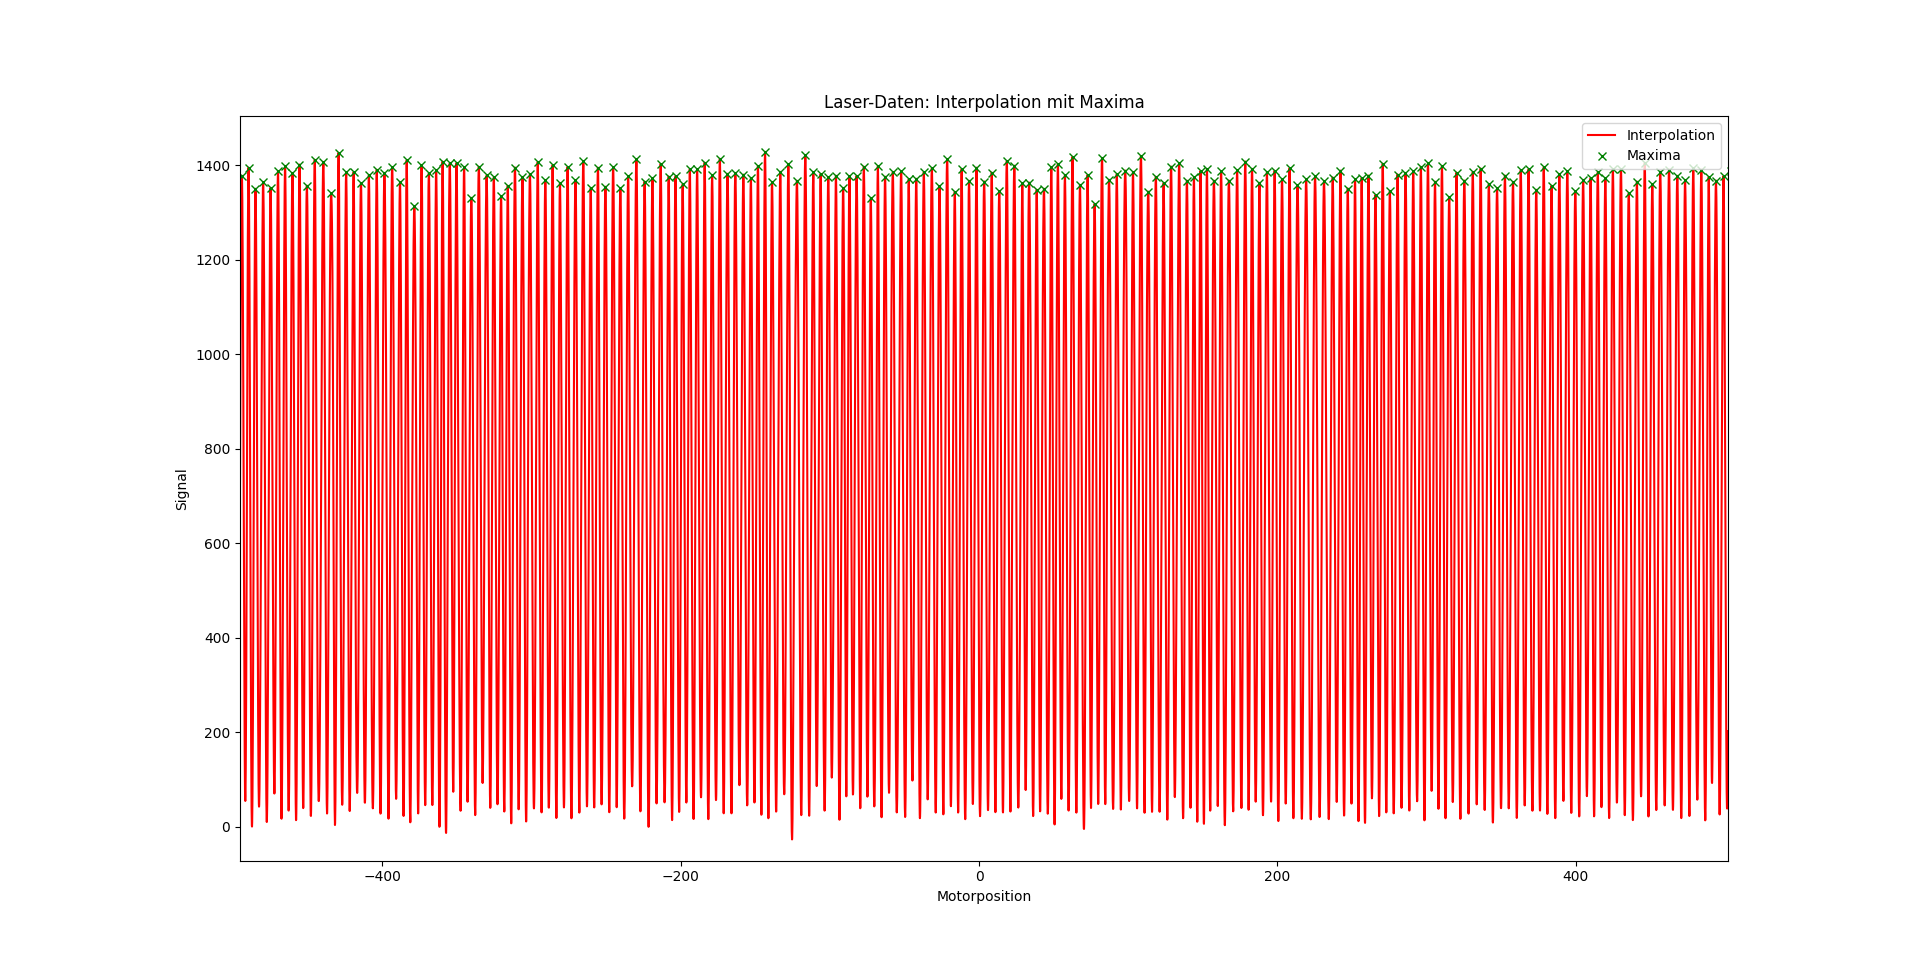
\includegraphics[width=1\linewidth]{img/Laser Daten Interpolation mit Maxima (zoom).png}
       \caption{Nach der Maximabestimmung: Maxima (grüne x) überlagert mit den interpolierten Laserdaten (rot).}
       \label{fig:LaserDatenInterpolationmitMaxima}
\end{figure}

\begin{figure}[H]
       \centering
       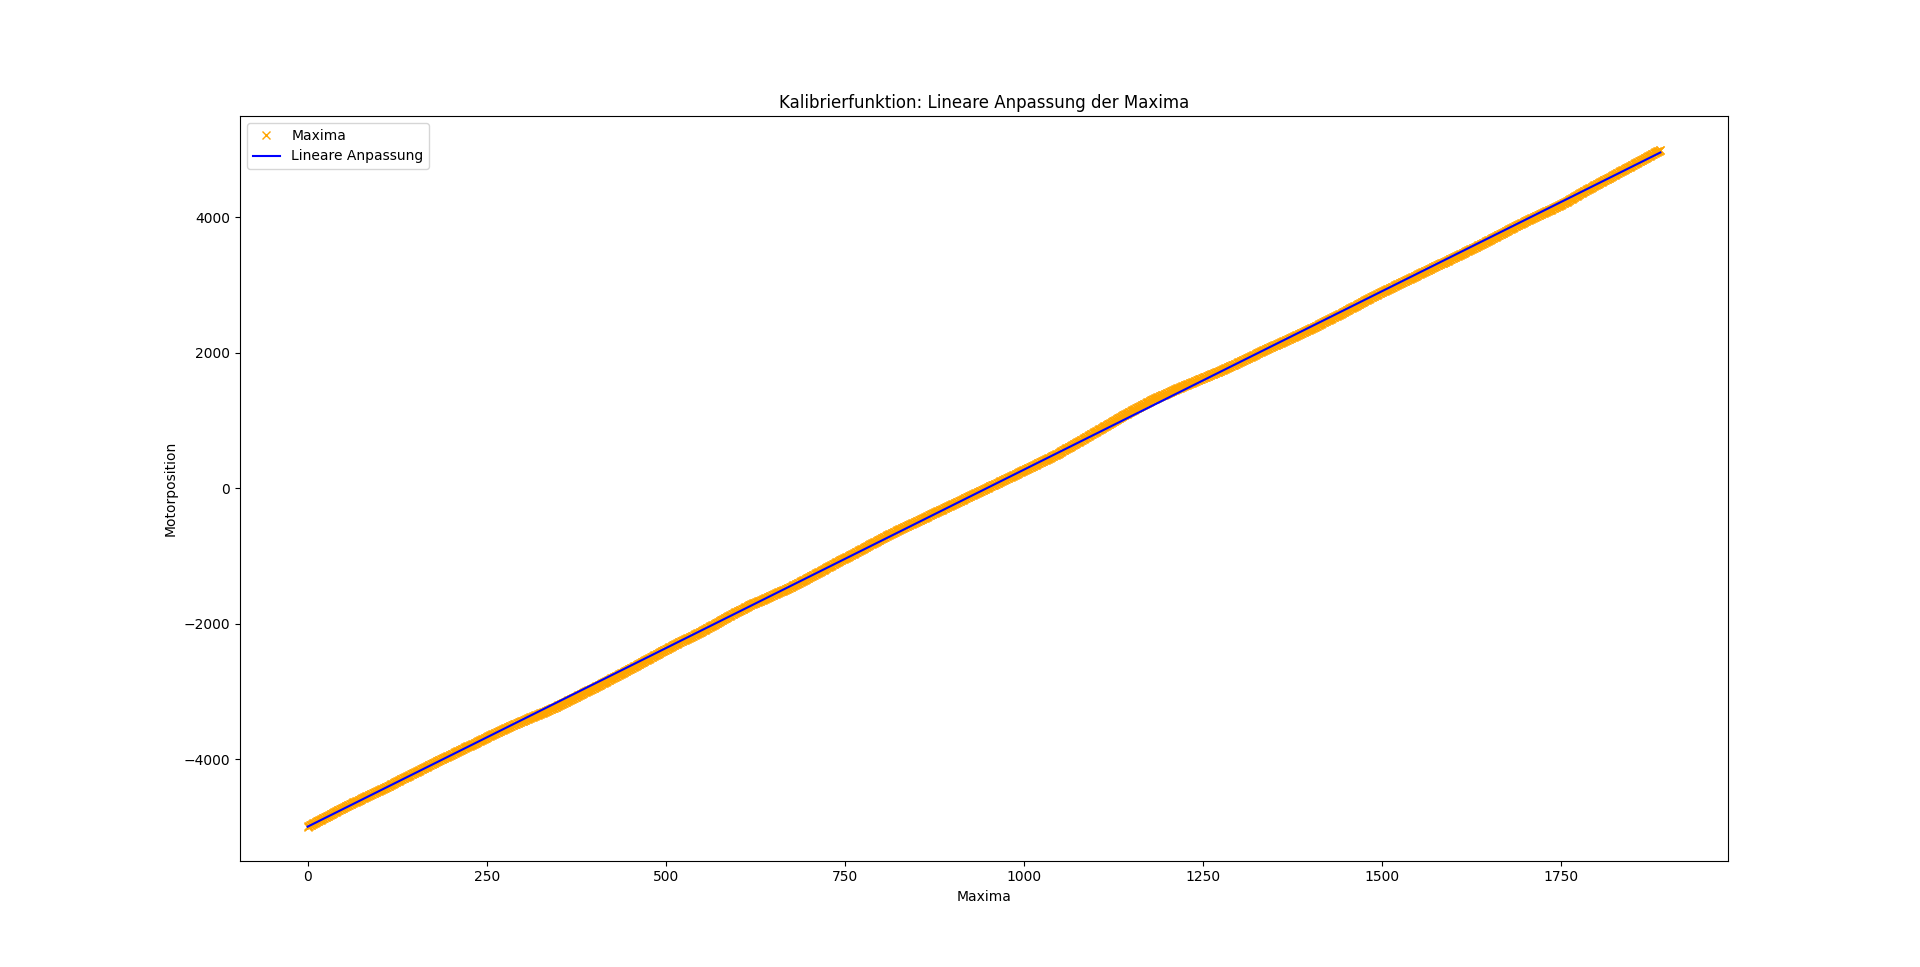
\includegraphics[width=1\linewidth]{img/Kalibrierfunktion.png}
       \caption{Der linerare Fit der Extrema (Soll Position, blaue Linie) im Vergleich zu den Ist Positionen der Maxima (gelbe x).}
       \label{fig:Kalibrierfunktion}
\end{figure}

\begin{figure}[H]
       \centering
       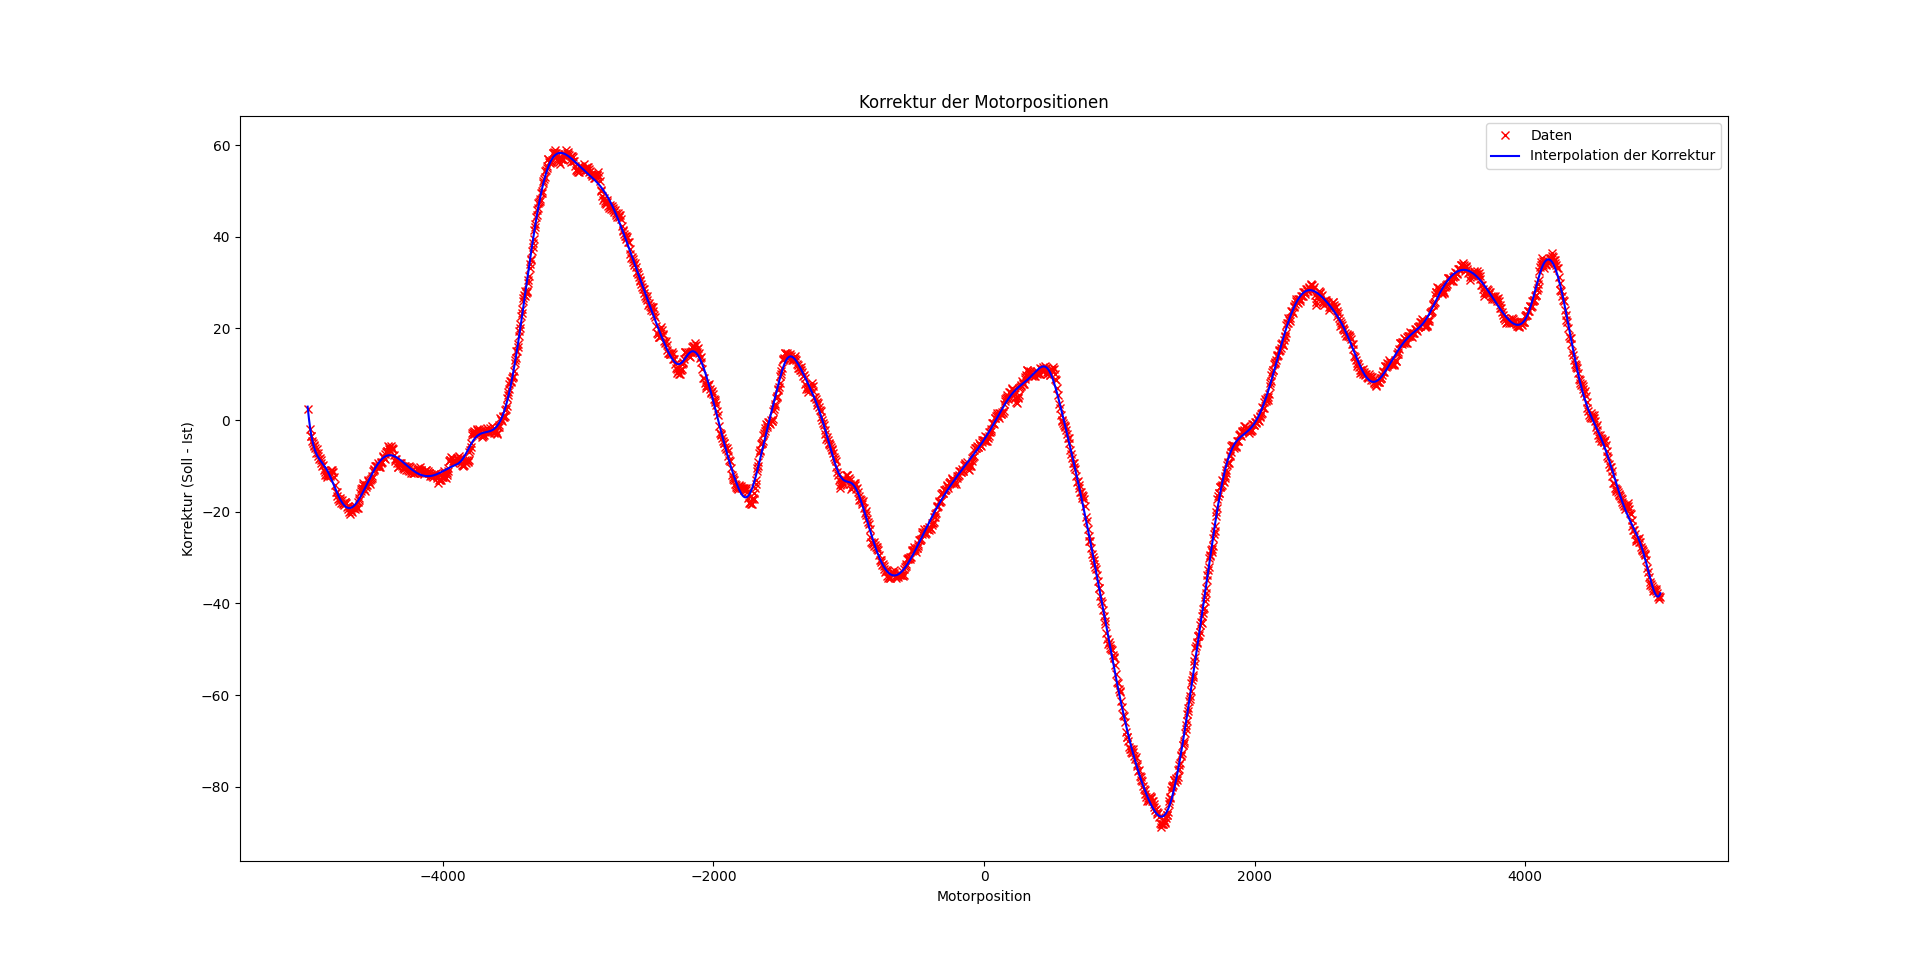
\includegraphics[width=1\linewidth]{img/Korrektur der Motorposition.png}
       \caption{Korrektur der Motorposition mit dem errechneten Delta (Soll Position - Ist Position).}
       \label{fig:KorrekturderMotorposition}
\end{figure}


\subsection{Korrektur der Weißlichtdaten und äquidistantes Gitter}

Nachdem die jeweilige Korrekturfunktion anhand der Laserdaten bestimmt wurde, erfolgt im nächsten Schritt die Linearisierung der Messdaten für die Jod-Probe und die Referenzmessung (bzw. der Filter- und Weißlichtmessung). Dieser Prozess ist entscheidend, um die mechanischen Unzulänglichkeiten des Verschiebetisches rechnerisch zu kompensieren und eine valide Basis für die Spektralanalyse zu schaffen.

\begin{itemize}
       \item Ortskorrektur der Weißlichtdaten: Zur Korrektur der ursprünglichen Ortsachse wird für jede Motorposition der entsprechende Korrekturwert aus der zuvor berechneten Kalibrierfunktion $\Delta(i)$ ermittelt und auf die jeweilige „Ist-Position“ addiert ($x_{korr}=x_{ist}+\Delta(x_{ist})$). Durch diese Transformation wird die nicht-lineare Bewegung des Schrittmotors begradigt, sodass die korrigierten Positionswerte den tatsächlichen optischen Weglängendifferenzen im Interferometer entsprechen.
       \item Erzeugung eines äquidistanten Gitters: Eine zwingende mathematische Voraussetzung für die Durchführung der diskreten Fouriertransformation (FFT) ist eine streng äquidistante Abtastung des Signals. Da die Ortsachse nach der Addition der Korrekturwerte zwar linearisiert, aber die Abstände zwischen den Punkten nun ungleichmäßig verteilt sind, müssen die Datenpunkte neu angeordnet werden.
       \item Interpolation auf eine gemeinsame Basis: Um die Proben- und Referenzdaten später physikalisch miteinander verrechnen zu können (z. B. für die Bestimmung der optischen Dichte), müssen beide Datensätze auf ein exakt identisches und äquidistantes Gitter transformiert werden. Hierzu wird ein gemeinsamer Ortsbereich definiert, der den überlappungsbereich beider Messungen abdeckt. Die gemittelten Amplitudenwerte werden anschließend mittels einer erneuten Spline-Interpolation den neuen, gleichmäßig beabstandeten Stützstellen zugeordnet.
\end{itemize}

Dieser Schritt stellt sicher, dass die resultierenden Spektren nach der Transformation im Frequenzraum präzise aufeinanderliegen und apparative Einflüsse durch die Verrechnung mit dem Referenzstrahlengang effektiv eliminiert werden können.

\subsubsection{Ortskorrektur Code}

\begin{lstlisting}[language=Python, caption=Ortskorrektur]
def ortskorrektur(positions, values, delta_interpolate):
       # Ursprüngliche Achse korrigieren
       x_korr = positions + delta_interpolate(positions)
       
       # Erzeugen eines äquidistanten Gitters für die FFT
       x_eq = np.linspace(x_korr.min(), x_korr.max(), len(x_korr))
       
       # Erneute Interpolation auf das neue Gitter
       f_int = make_interp_spline(x_korr, values, k=3)
       y_eq = f_int(x_eq)
       
       return x_eq, y_eq
\end{lstlisting}

\subsection{Transformation in den Zeit- und Frequenzraum}


Nachdem die Messdaten erfolgreich ortskorrigiert und auf ein äquidistantes Gitter transformiert wurden, erfolgt der übergang von der räumlichen Domäne in die zeitliche Verzögerung und schließlich in den Frequenzraum.

\begin{itemize}
       \item Transformation der Ortsachse in die Zeitverzögerung $\Delta t$: Die korrigierte Motorachse $x_{\text{korr}}$ liegt zunächst in Einheiten von Motorschritten vor. Um eine physikalisch interpretierbare Zeitachse zu erhalten, wird die präzise bekannte Wellenlänge des Kalibrierlasers ($\lambda_L = \qty{532}{nm}$) herangezogen. Da der Abstand zwischen zwei Intensitätsmaxima im Interferogramm einer Änderung der optischen Weglängendifferenz um exakt $\lambda_L$ entspricht, lässt sich über die Steigung $a$ der Laserkalibrierung (Motorschritte pro Maximum) die geometrische Weglängendifferenz $\Delta s$ berechnen. Unter Berücksichtigung der Lichtgeschwindigkeit $c$ wird diese in die zeitliche Verzögerung $\Delta t$ der Teilstrahlen überführt: $$\Delta t = \frac{\Delta s}{c} = \frac{x_{\text{korr}} \cdot \lambda_L}{a \cdot c}.$$ Diese äquidistante Zeitachse bildet die notwendige Basis für die diskrete Fouriertransformation.
       \item Spektralanalyse via Fouriertransformation: Die physikalische Grundlage für die Extraktion der spektralen Informationen bildet das Wiener-Khinchin-Theorem. Dieses besagt, dass das gemessene Interferogramm $\Delta I(\Delta t)$ mathematisch der Autokorrelationsfunktion des elektrischen Feldes entspricht und somit die Fouriertransformierte der spektralen Energiedichte $W(\omega)$ darstellt. Für die numerische Berechnung im Skript werden die Funktionen `fft` und `fftshift` aus der SciPy-Bibliothek verwendet:
       \begin{itemize}
              \item 'fft' (Fast Fourier Transform): Transformiert das zeitliche Signal in den komplexen Frequenzraum. Um physikalisch korrekte Amplituden zu erhalten, wird das Resultat durch die Anzahl der Datenpunkte $N$ normiert.
              \item 'fftshift': Da der FFT-Algorithmus die Frequenzen standardmäßig in einer Reihenfolge ausgibt, die bei der Nullfrequenz beginnt, verschiebt diese Funktion die Frequenzkomponenten so, dass die Nullfrequenz in der Mitte des Arrays liegt. Dies ermöglicht eine intuitive Darstellung des symmetrischen Spektrums von $-f_{\text{Nyquist}}$ bis $+f_{\text{Nyquist}}$.
       \end{itemize}
       \item Sampling und Auflösungsgrenze: In diesem Schritt wird zudem die Abtastrate $T_{\text{sampl}}$ (zeitlicher Abstand zwischen zwei Messpunkten) definiert. Gemäß dem Nyquist-Shannon-Abtast- theorem begrenzt diese die maximal auflösbare Frequenz des Spektrometers ($f_{\text{max}} = 1 / (2 \cdot T_{\text{sampl}})$). Die theoretische spektrale Auflösung $\Delta \nu$ hingegen ist durch die maximale zeitliche Verzögerung $\Delta t_{\text{max}}$ begrenzt, die während des Scans erreicht wurde ($\Delta \nu = 1 / \Delta t_{\text{max}}$).
\end{itemize}

\subsubsection{FFT Code}

\begin{lstlisting}[language=Python, caption=FFT]
def fft_spectrum(x_eq, y_eq, laser_slope):
       """
       Führt die Ort-zu-Zeit Transformation und die FFT durch.
       
       Parameter:
       x_eq: Äquidistante Ortsachse (Motorschritte)
       y_eq: Interpolierte Signalwerte (Kanal 0, 1 oder 2)
       laser_slope: Steigung aus der Laserkalibrierung (Schritte pro Maximum)
       """
       # Ort zu Zeit Transformation
       #lambda_half = 266e-9 
       delta_s = (x_eq * 532e-9) / laser_slope
       delta_t_axis = delta_s / c
   
       # Sampling-Parameter für die FFT
       # Wir benötigen das Zeitintervall T_sampl als Skalar für die Frequenzachse.
       L = len(delta_t_axis)
       t_range = np.max(delta_t_axis) - np.min(delta_t_axis)
       
       # Tsampl oft in Ts angegeben (Faktor 1e12), um handliche Frequenzwerte zu erhalten.
       T_sampl = (t_range / L)  * 1e12
       f_max = 1 / T_sampl
       f_ny = f_max / 2
       
       # Frequenzachse erzeugen
       # Die FFT liefert ein symmetrisches Signal um die Frequenz 0.
       freq_axis = np.linspace(-f_ny, f_ny, L)
   
       # FFT berechnen und verschieben
       # Division durch L reduziert die Signalamplitude auf physikalisch sinnvolle Werte.
       spectrum_raw = fft(y_eq / L)
       spectrum_shifted = fftshift(spectrum_raw)
       spectrum_abs = np.abs(spectrum_shifted)
   
       return freq_axis, spectrum_abs
\end{lstlisting}

\subsection{Berechnung von OD und DOT}

Um die spezifischen Absorptionsmerkmale der untersuchten Proben – des Notch-Filters und der Iod-Küvette – präzise vom Emissionsprofil der Lichtquelle zu trennen, wird das Probenspektrum $I$ mit einem simultan aufgenommenen Referenzspektrum $I_0$ der reinen Weißlicht-LED verglichen. Da das Spektrum der LED kein flaches Plateau aufweist, sondern durch charakteristische Maxima (z. B. den Blaulicht-Peak bei ~\qty{450}{nm}) und apparative Artefakte wie „spektrale Löcher“ (bei ca. \qty{604}{nm} und \qty{617}{nm}) geprägt ist, ist diese Normierung essenziell, um echte Absorptionseffekte zu isolieren.

Für die grafische Darstellung und quantitative Analyse werden zwei komplementäre Größen berechnet:
\begin{itemize}
       \item Optische Dichte (OD): Die optische Dichte beschreibt die Abschwächung des Lichts beim Durchgang durch die Probe auf einer logarithmischen Skala: $$OD = -\log_{10}\left(\frac{I}{I_0}\right)$$ Diese Darstellung eignet sich besonders für die Analyse der Iod-Küvette. Sie macht die feinen, oft eng beieinander liegenden Molekülübergänge (Vibrationsübergänge) im gelb-grünen Spektralbereich sichtbar, die im Rohspektrum aufgrund des geringen Signal-zu-Rausch-Verhältnisses und der starken Gesamtabsorption oft schwer aufzulösen sind.
       \item Differentielle optische Transmission (DOT): Die DOT stellt die relative Intensitätsänderung im Vergleich zur Referenz dar: $$DOT = \frac{I - I_0}{I_0}$$ Diese Metrik wird bevorzugt zur Charakterisierung des Interferenzfilters (Notch-Filter) herangezogen. Durch die DOT-Darstellung lassen sich die Zentralwellenlänge (ca. \qty{515}{nm}) und die spektrale Bandbreite des Filters präzise bestimmen, da die Filterkurve hierbei direkt als Abweichung von der Nulllinie erscheint.
\end{itemize}
Durch die Anwendung dieser Korrekturverfahren können subtile Details in den Spektren hervorgehoben werden, die andernfalls durch die spektrale Verteilung der LED überlagert würden. Dies ermöglicht letztlich die experimentelle Bestätigung theoretischer Erwartungen, wie etwa der äquidistanten Absorptionslinien des zweiatomigen Iod-Moleküls.

\section{Diskussion der physikalischen Ergebnisse}

\subsection{Spektren}
\subsubsection{Laser}
\begin{figure}[!h]
	\centering
	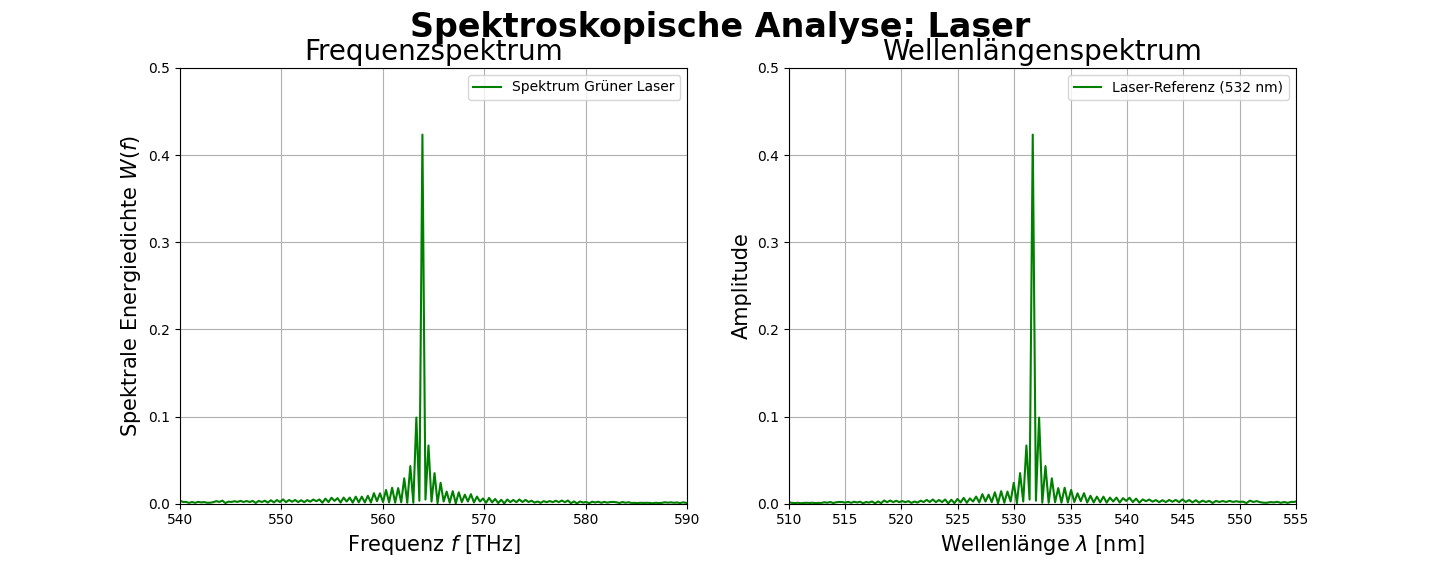
\includegraphics[width=1\linewidth]{img/Spektrum Laser 1 final.png}
	\caption{Ausschnitt des Laserpektrums in Abhängigkeit der Wellenlänge}
	\label{fig: laserspek}
\end{figure}
Von dem experimentell bestimmten Laserspektrum (siehe \autoref{fig: laserspek}), lässt sich eine Wellenlänge von \qty{532,01}{nm} ablesen. Diese entspricht der tatsächlichen Wellenlänge des Lasers $\lambda_L=\qty{532}{nm}$ und zeugt von einer korrekten Kalibrierfunktion, die auch für die weiteren Messwerte angewendet werden kann.

\subsubsection{Interferenz-Filter}
\begin{figure}[!h]
	\centering
	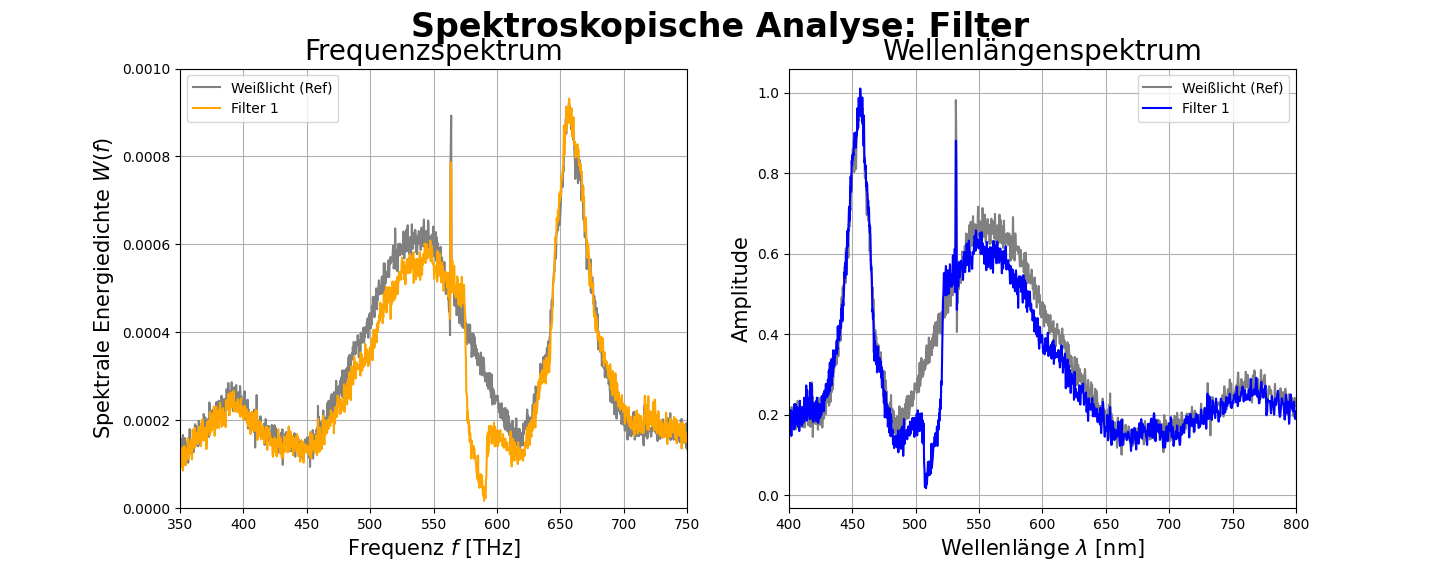
\includegraphics[width=1\linewidth]{img/Spektrum Filter 1 final.png}
	\caption{Das gemessene Spektrum des Filters in Abhängigkeit von Frequenz und Wellenlänge dargestellt und verglichen mit dem Referenzspektrum der Weißlichtquelle}
	\label{fig: filter2spek}
\end{figure}
Das Spektrum des Interferen-Filters weicht hauptsächlich in den Intensitäten von dem Referenzspektrum ab (siehe \autoref{fig: filter2spek}). Die genaueren Abweichungen lassen sich an der differentiellen optischen Transmission des Filters erkennen (siehe \autoref{fig: filter2dot}).\\
\begin{figure}[!h]
	\centering
	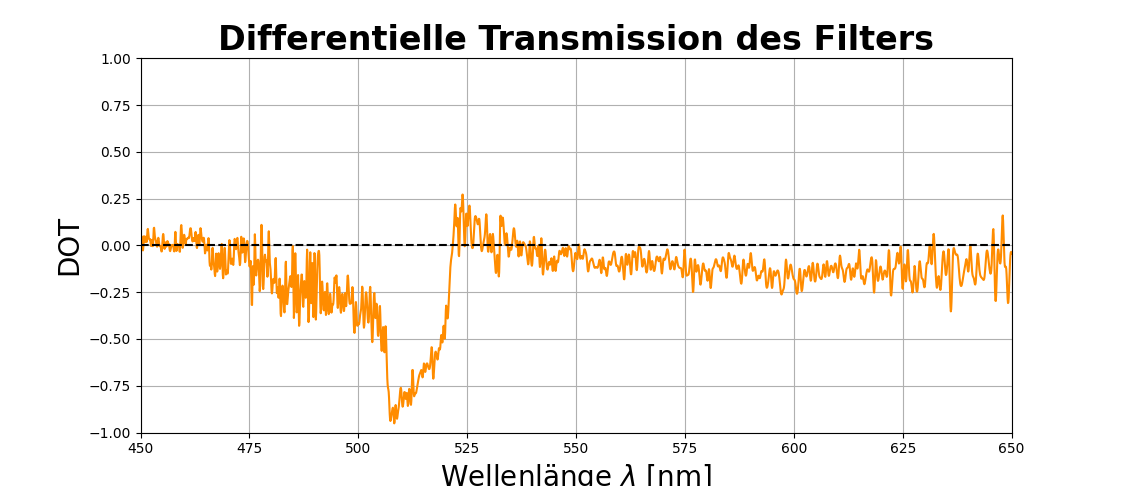
\includegraphics[width=1\linewidth]{img/Differentielle Transmission Filter 1 final.png}
	\caption{Die differentielle Transmission des Filters bestimmt durch das Referenzspektrum der Weißlichtquelle}
	\label{fig: filter2dot}
\end{figure}
Auffällig sind hier vor allem die starke Absorption in einem Wellenlängenbereich von etwa \qtyrange{495}{520}{\nm}. Der Filter filtert also grünes Licht in einem schmalen Bereich, was für einen schmalbandigen Interferenz-Filter spricht.\\\\
Die spektrale Bandbreite $B$ des Filters lässt sich mithilfe der DOT in Frequenzdarstellung bestimmen:
$$B=f_{max}-f_{min}=\frac{c}{\lambda_{min}}-\frac{c}{\lambda_{max}}=\frac{c}{493\si{\nm}}-\frac{c}{521\si{\nm}}=\qty{32,68}{\peta\hertz}$$
Die Zentralwellenlänge $\lambda_Z$ liegt bei $\lambda_Z=\frac{c}{f_min+\frac{B}{2}}=\qty{506,6}{\nm}$. 

\subsubsection{Iod-Küvette}
\begin{figure}[!h]
	\centering
	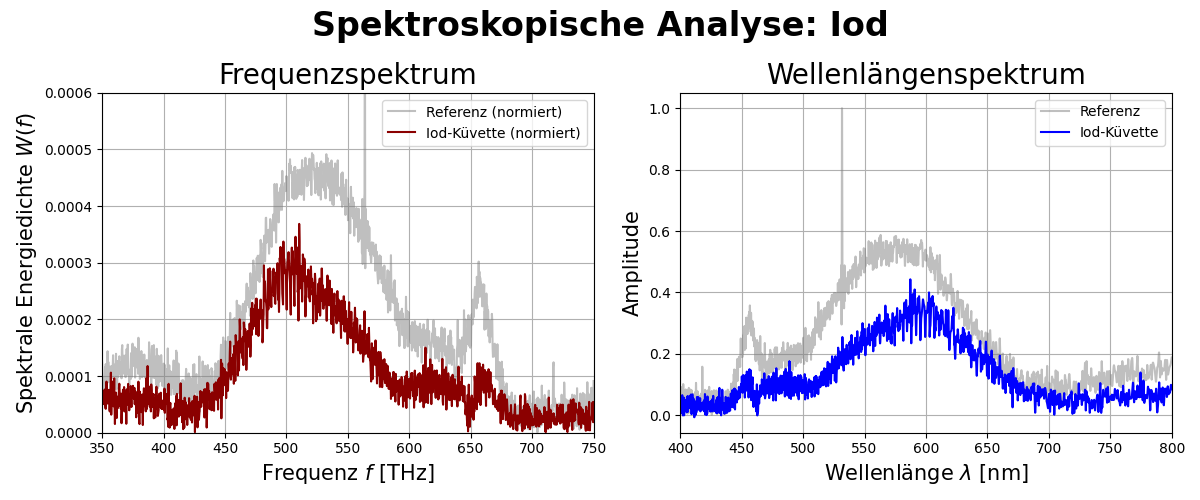
\includegraphics[width=1\linewidth]{img/Spektrum Iod 1 final.png}
	\caption{Das gemessene Iod-Spektrum in Abhängigkeit von Frequenz und Wellenlänge dargestellt und verglichen mit dem Referenzspektrum der Weißlichtquelle gemessen durch eine leere Küvette}
	\label{fig: iod2spek}
\end{figure}
\begin{figure}[h]
	\centering
	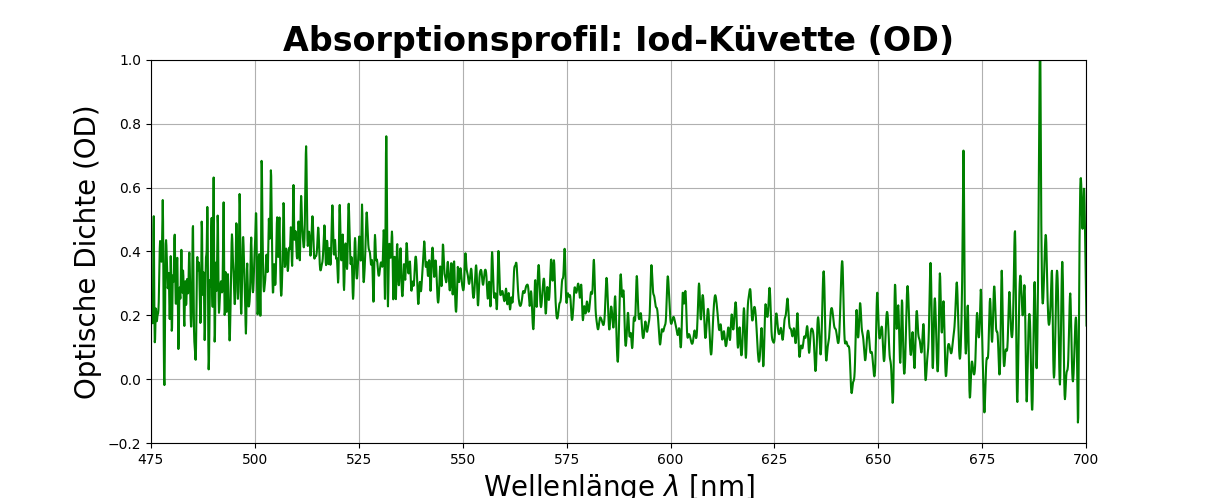
\includegraphics[width=1\linewidth]{img/Absorsptionsprofil Iod 1 OD final.png}
	\caption{Die optische Dichte des Iod-Spektrums bestimmt durch das Referenzspektrum einer leeren Küvette}
	\label{fig: iod2od}
\end{figure}
Bei der Betrachtung des Iod-Spektrums (siehe \autoref{fig: iod2spek}) ist zu sehen, dass das Referenzspektrum der leeren Küvette deutlich mehr Rauschen enthält. Das Rauschen, was bei dem Spektrum der Iod-Küvette zu sehen ist, ist außerdem gleichförmiger. Wie auch am Absorptionsprofil erkennbar, dargestellt durch die optische Dichte (siehe \autoref{fig: iod2od}), wird durch das Iod unter anderem sehr viel von dem Rauschen absorbiert.\\
Die gemessene Intensität ist außerdem bei dem Iod-Spektrum in einem Wellenlängenbereich von ca. \qtyrange{420}{670}{nm} deutlich geringer als das Referenzspektrum, da Iod im Allgemeinen kurzwelliges Licht stärker absorbiert, als langwelliges Licht.
\\\\
Das gemessene Iod-Spektrum passt zu Iod-Spektren, die in einer anderen Studie gemessen wurden (siehe \autoref{fig: iodlit}) \cite{4}.\\
Das Maximum befindet sich im gleichen Wellenlängenbereich und hat eine ähnliche Form. Die kleineren Peaks entlang der Kurve unterscheiden sich leicht in Form, zeigen aber beide die Emissions- bzw. Absorptionsspektrallinien charakteristisch für Iod.\\\\
\begin{figure}[h]
	\centering
	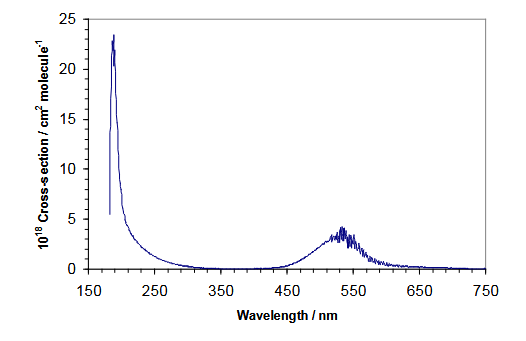
\includegraphics[width=0.5\linewidth]{img/iod literatur2.png}
	\caption{Gemessener $I_2$ Absorptionsquerschnitt \cite{4}}
	\label{fig: iodlit}
\end{figure}
Bei genauerer Betrachtung der optischen Dichte der Iod-Küvette lassen sich viele klare Maxima erkennen. Diese spiegeln das Absorptionsspektrum von Iod wieder. Jedes Maximum repräsentiert eine Spektrallinie, die bei Iod im Bereich \qtyrange{500}{700}{nm} in hoher Anzahl auftreten. Das sind die Vibrationsübergänge des Moleküls. Das experimentell bestimmte Spektrum passt zu der theoretischen Erwartung (siehe \autoref{fig: iodtheo}). 
\begin{figure}[h]
	\centering
	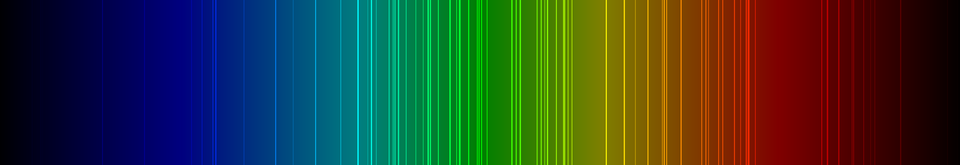
\includegraphics[width=0.75\linewidth]{img/960px-Iodine_spectrum_visible.png}
	\caption{Das sichtbare Spektrum von Iod \cite{3}}
	\label{fig: iodtheo}
\end{figure}

\subsection{Spektrale Auflösung}
Die theoretische Auflösungsgrenze des Fourier-Transform-Spektrometers lässt sich bestimmen durch die Wegzeitdifferenz $\Delta t$. Da der benutzte Schrittmotor eine kleinstmögliche Verschiebung von \qty{50,5}{\nm} hat und wir 10000 Schritte pro Messreihe gelaufen sind, ist unsere Weglängendifferenz $\Delta s = 10000 \cdot 50,5 \cdot 10^{-9} \cdot 2 = \qty{1,01}{\mm}$.
Daraus lässt sich $\Delta t = \frac{1,01 \cdot 10^{-3}}{c} = \qty{3,37}{\pm}$ bestimmen.\\
Die theoretische spektrale Auflösungsgrenze ist dann:
$$\Delta\nu=\frac{1}{\Delta t}=\qty{0,297}{\peta\hertz}=\qty{1.009e-3}{\nm}$$
\\
Experimentell lässt sich eine Signalbreite von \qty{0,6}{\peta\hertz} aus dem Laserspektrum ablesen. Die Auflösung im Experiment ist 50\% größer als die theoretische Auflösungsgrenze.

\subsection{Fehlerdiskussion}
Bei dem experimentellen Aufbau gibt es mehrere Fehlerquellen. Die Interpolation der Laserdaten zum Aufbauen der Kalibrierfunktion ist eine der grundlegenden, da das Signal des Lasers Schwankungen hat, die sich durch alle restlichen Ergebnisse fortpflanzen. Das würde auch heißen, dass die Linienbreite des Lasers größer ist als angenommen, das Experiment hat also eine schlechtere Auflösung, als jetzt bestimmt.

Einer der größten systematischen Fehler in diesem Experiment ist die Nichtlinearität des Schrittmotors. Zur Kompensation dieses Fehlers wird in der Datenanalyse eine Kalibrierfunktion angewendet. Da die Spektren grundsätzlich den theoretischen Erwartungen entsprechen, ist davon auszugehen, dass die Korrektur erfolgreich durchgeführt wurde. Diese Annahme wird zudem durch den Vergleich des Lasersignals mit der korrigierten Ortsachse und dem ursprünglich interpolierten Signal gestützt (siehe \autoref{fig: korrvgl}).
\begin{figure}[H]
	\centering
	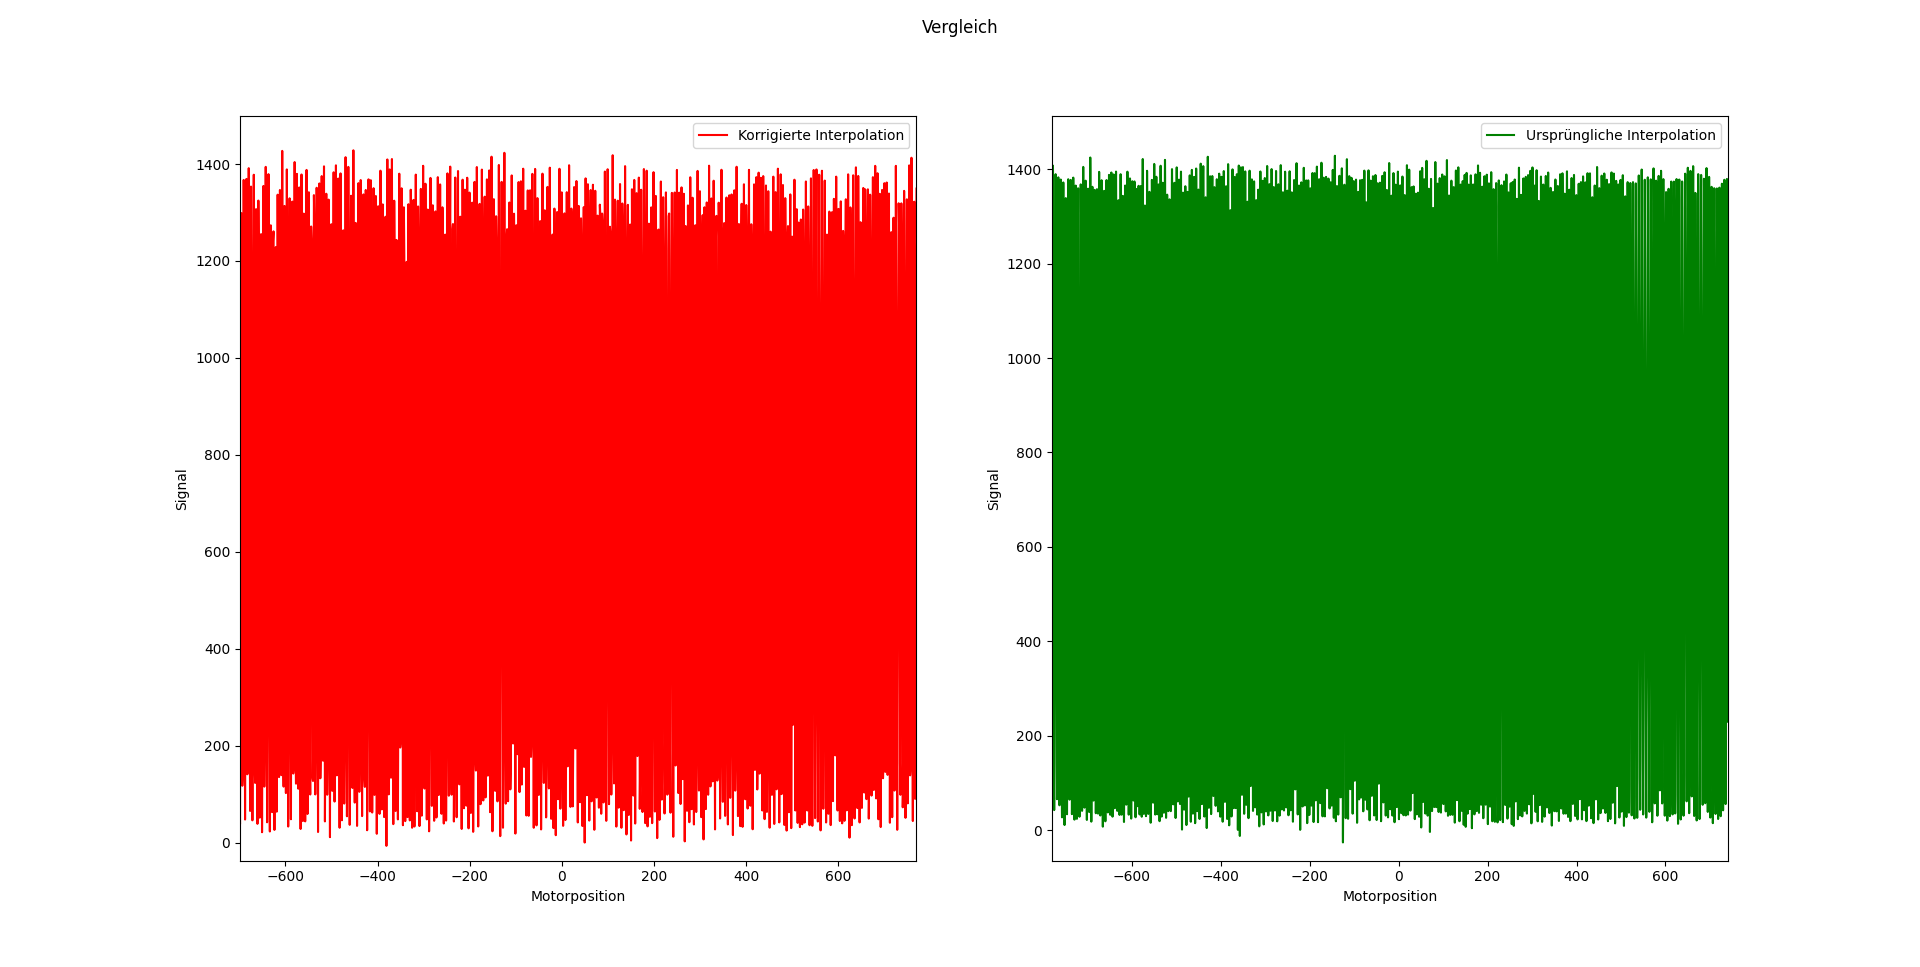
\includegraphics[width=0.9\linewidth]{img/Vergleich Ursprüngliche vs Korrigierte Interpolation.png}
	\caption{Vergleich zwischen der ursprünglichen Interpolation der Laserdaten und der Interpolation mit korrigierter Ortsachse}
	\label{fig: korrvgl}
\end{figure}
\\\\
Für jede Probe wurden jeweils zwei Messreihen durchgeführt.\\ %Die Ergebnisse der ersten Messreihen entsprechen den theoretischen Erwartungen weniger gut als die der zweiten Messreihen. Dies deutet auf einen erheblichen systematischen Fehler hin, da die Auswertungsmethode bei allen Datensätzen einheitlich angewendet wurde. In der vorliegenden Auswertung sind daher die Ergebnisse der zweiten Messreihen dargestellt.
\begin{figure}[H]
	\centering
	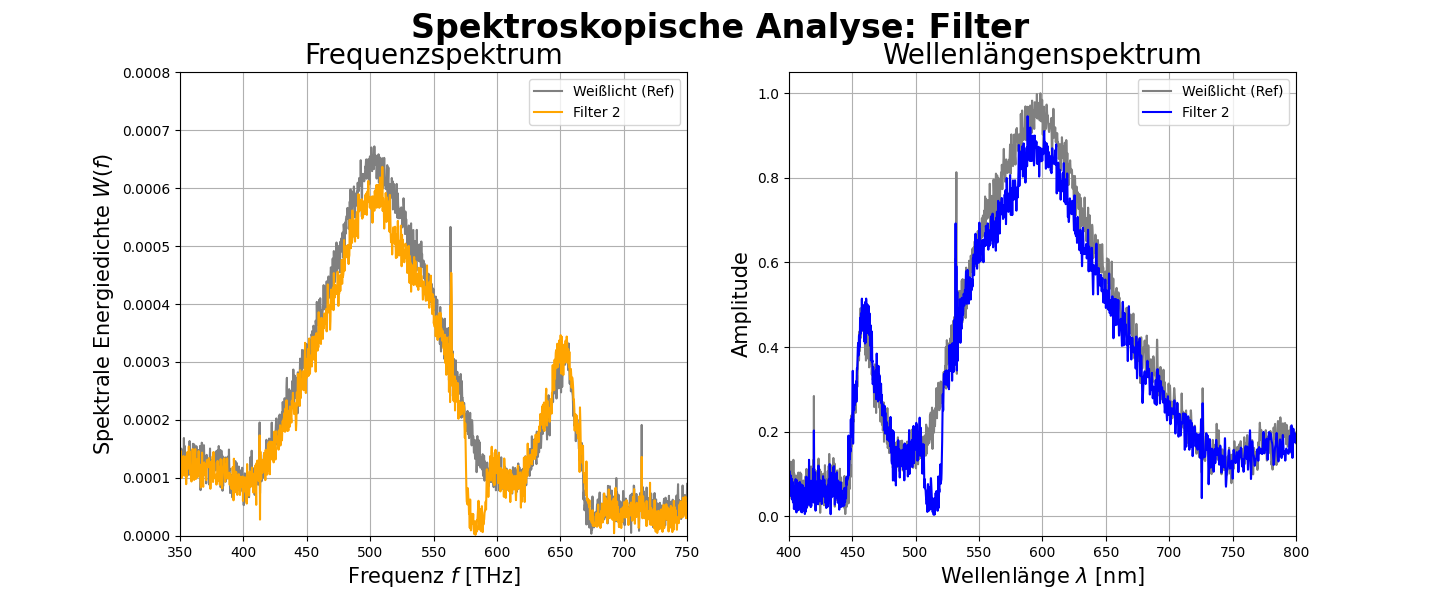
\includegraphics[width=1\linewidth]{img/Spektrum Filter final.png}
	\caption{Das in Messreihe 2 gemessene Spektrum des Filters in Abhängigkeit von Frequenz und Wellenlänge dargestellt und verglichen mit dem Referenzspektrum der Weißlichtquelle}
	\label{fig: filter1spek}
\end{figure}
\begin{figure}[H]
	\centering
	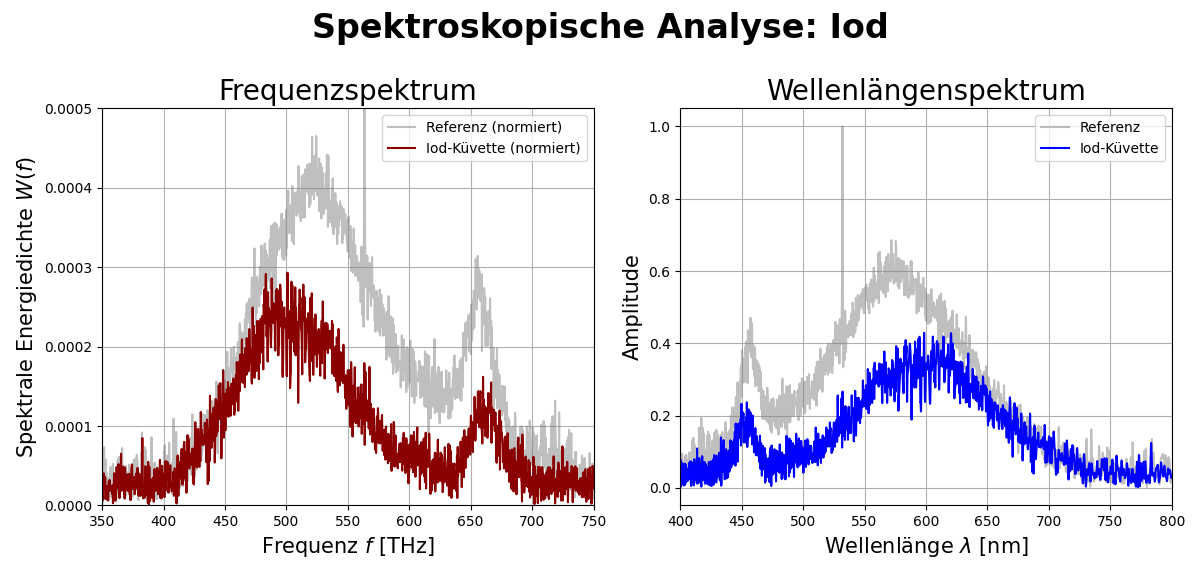
\includegraphics[width=1\linewidth]{img/Spektrum Iod final.png}
	\caption{Das in Messreihe 2 gemessene Iod-Spektrum in Abhängigkeit von Frequenz und Wellenlänge dargestellt und verglichen mit dem Referenzspektrum der Weißlichtquelle gemessen durch eine leere Küvette}
	\label{fig: iod1spek}
\end{figure}
%Bei den ersten Messreihen fallen die Intensitäten sowie das Rauschen der Spektren deutlich stärker aus (\autoref{fig: filter1spek} und \autoref{fig: iod1spek}). Zwischen den beiden Messdurchgängen wurde das Spektrometer neu justiert und die Nullposition des Motors neu eingestellt. Es lässt sich daraus schließen, dass die Erstjustage qualitativ etwas ungenauer war. Zudem ist zwischen der ersten Justierung und den ersten Messreihen mehr Zeit vergangen als zwischen der zweiten Justierung und den zweiten Messreihen. Dadurch hatte das Spektrometer mehr Gelegenheit, sich durch äußere Einflüsse zu verändern, beispielsweise durch Temperaturschwankungen im Raum, kleine Vibrationen des Tisches oder das Ein- und Austreten aus dem Raum beim Probenaustausch.

\section{Zusammenfassung}

Im Rahmen des Versuchs KV6 wurde die Fourier-Transform-Spektroskopie (FTS) im sichtbaren Spektralbereich untersucht. Ziel des Experiments war die Bestimmung des Emissionsspektrums einer Weißlicht-LED sowie der Absorptionsspektren eines Interferenzfilters und einer mit Iod gefüllten Küvette.\\\\
Die methodische Grundlage bildete die Vermessung der zeitlichen Kohärenzfunktion (Autokorrelationsfunktion) mithilfe eines Michelson-Interferometers. Da die mechanische Bewegung des Linearverschiebetisches keine exakte Linearität aufwies, wurde eine numerische Kalibrierfunktion basierend auf einem simultan aufgenommenen Laser-Interferogramm ($\lambda_L=\qty{532}{\nm}$) erstellt. Mithilfe einer in Python programmierten Auswerteroutine wurden die Messdaten ortskorrigiert, äquidistanziert und schließlich mittels Fouriertransformation in den Frequenzraum überführt.\\\\
Die physikalische Auswertung ergab folgende Resultate:
\begin{itemize}
       \item Für den Interferenzfilter wurde eine Zentralwellenlänge von ca. \qty{506,6}{\nm} bei einer spektralen Bandbreite von \qty{9,18}{\nm} ermittelt.
       \item In den Iodspektren konnten die charakteristischen Absorptionslinien aufgelöst und als Vibrationsübergänge des Moleküls verifiziert werden.
       \item Die experimentell bestimmte spektrale Auflösung lag mit ca. \qty{0,6}{\peta\hertz} in der Größenordnung der theoretischen Auflösungsgrenze von \qty{0,297}{\peta\hertz}.
\end{itemize}
Trotz verbleibender systematischer Unsicherheiten, insbesondere durch die Nichtlinearität des Schrittmotors und thermische Instabilitäten, konnte das Funktionsprinzip der Fourier-Spektroskopie erfolgreich demonstriert und die Eignung der numerischen Datenkorrektur bestätigt werden.

\newpage
\pagenumbering{Alph}


\bibliographystyle{ieeetr}
\bibliography{praktikum}

\newpage

\listoffigures %lof
\addcontentsline{toc}{section}{Abbildungsverzeichnis}

\newpage

\begin{appendices}
\section{Code}
%\lstinputlisting[language=Python]{KV6 Aufgeräumt.py}

\end{appendices}


\end{document} 
